\documentclass{anstrans}
%%%%%%%%%%%%%%%%%%%%%%%%%%%%%%%%%%%
\title{Demonstration of Demand Driven Deployment Capabilities in \Cyclus}
\author{Gwendolyn J. Chee$^1$, Jin Whan Bae$^1$, Robert R. Flanagan$^2$, Roberto E. Fairhurst$^1$ and Kathryn D. Huff$^1$}

\institute{
$^1$Dept. of Nuclear, Plasma and Radiological Engineering, University of Illinois at Urbana-Champaign \\
$^2$Nuclear Engineering Program, University of South Carolina \\

gchee2@illinois.edu
}

%%%% packages and definitions (optional)
\usepackage{graphicx} % allows inclusion of graphics
\usepackage{booktabs} % nice rules (thick lines) for tables
\usepackage{microtype} % improves typography for PDF
\usepackage{xspace}
\usepackage{tabularx}
\usepackage{subcaption}
\usepackage{enumitem}
\usepackage{placeins}
\usepackage{multirow}
\usepackage[acronym,toc]{glossaries}
%\newacronym{<++>}{<++>}{<++>}
\newacronym[longplural={metric tons of heavy metal}]{MTHM}{MTHM}{metric ton of heavy metal}
\newacronym{ABM}{ABM}{agent-based modeling}
\newacronym{ACDIS}{ACDIS}{Program in Arms Control \& Domestic and International Security}
\newacronym{AHTR}{AHTR}{Advanced High Temperature Reactor}
\newacronym{ANDRA}{ANDRA}{Agence Nationale pour la gestion des D\'echets RAdioactifs, the French National Agency for Radioactive Waste Management}
\newacronym{ANL}{ANL}{Argonne National Laboratory}
\newacronym{API}{API}{application programming interface}
\newacronym{ARE}{ARE}{Aircraft Reactor Experiment}
\newacronym{ARFC}{ARFC}{Advanced Reactors and Fuel Cycles}
\newacronym{ASME}{ASME}{American Society of Mechanical Engineers}
\newacronym{ATWS}{ATWS}{Anticipated Transient Without Scram}
\newacronym{BDBE}{BDBE}{Beyond Design Basis Event}
\newacronym{BIDS}{BIDS}{Berkeley Institute for Data Science}
\newacronym{CAFCA}{CAFCA}{ Code for Advanced Fuel Cycles Assessment }
\newacronym{CDTN}{CDTN}{Centro de Desenvolvimento da Tecnologia Nuclear}
\newacronym{CEA}{CEA}{Commissariat \`a l'\'Energie Atomique et aux \'Energies Alternatives}
\newacronym{CI}{CI}{continuous integration}
\newacronym{CNEN}{CNEN}{Comiss\~{a}o Nacional de Energia Nuclear}
\newacronym{CNERG}{CNERG}{Computational Nuclear Engineering Research Group}
\newacronym{COSI}{COSI}{Commelini-Sicard}
\newacronym{COTS}{COTS}{commercial, off-the-shelf}
\newacronym{CSNF}{CSNF}{commercial spent nuclear fuel}
\newacronym{CTAH}{CTAHs}{Coiled Tube Air Heaters}
\newacronym{CUBIT}{CUBIT}{CUBIT Geometry and Mesh Generation Toolkit}
\newacronym{CURIE}{CURIE}{Centralized Used Fuel Resource for Information Exchange}
\newacronym{DAG}{DAG}{directed acyclic graph}
\newacronym{DANESS}{DANESS}{Dynamic Analysis of Nuclear Energy System Strategies}
\newacronym{DBE}{DBE}{Design Basis Event}
\newacronym{DESAE}{DESAE}{Dynamic Analysis of Nuclear Energy Systems Strategies}
\newacronym{DHS}{DHS}{Department of Homeland Security}
\newacronym{DOE}{DOE}{Department of Energy}
\newacronym{DRACS}{DRACS}{Direct Reactor Auxiliary Cooling System}
\newacronym{DRE}{DRE}{dynamic resource exchange}
\newacronym{DSNF}{DSNF}{DOE spent nuclear fuel}
\newacronym{DYMOND}{DYMOND}{Dynamic Model of Nuclear Development }
\newacronym{EBS}{EBS}{Engineered Barrier System}
\newacronym{EDZ}{EDZ}{Excavation Disturbed Zone}
\newacronym{EIA}{EIA}{U.S. Energy Information Administration}
\newacronym{EPA}{EPA}{Environmental Protection Agency}
\newacronym{EP}{EP}{Engineering Physics}
\newacronym{FCO}{FCO}{Fuel Cycle Options}
\newacronym{FCT}{FCT}{Fuel Cycle Technology}
\newacronym{FEHM}{FEHM}{Finite Element Heat and Mass Transfer}
\newacronym{FEPs}{FEPs}{Features, Events, and Processes}
\newacronym{FHR}{FHR}{Fluoride-Salt-Cooled High-Temperature Reactor}
\newacronym{FLiBe}{FLiBe}{Fluoride-Lithium-Beryllium}
\newacronym{GDSE}{GDSE}{Generic Disposal System Environment}
\newacronym{GDSM}{GDSM}{Generic Disposal System Model}
\newacronym{GENIUSv1}{GENIUSv1}{Global Evaluation of Nuclear Infrastructure Utilization Scenarios, Version 1}
\newacronym{GENIUSv2}{GENIUSv2}{Global Evaluation of Nuclear Infrastructure Utilization Scenarios, Version 2}
\newacronym{GENIUS}{GENIUS}{Global Evaluation of Nuclear Infrastructure Utilization Scenarios}
\newacronym{GPAM}{GPAM}{Generic Performance Assessment Model}
\newacronym{GRSAC}{GRSAC}{Graphite Reactor Severe Accident Code}
\newacronym{GUI}{GUI}{graphical user interface}
\newacronym{HLW}{HLW}{high level waste}
\newacronym{HPC}{HPC}{high-performance computing}
\newacronym{HTC}{HTC}{high-throughput computing}
\newacronym{HTGR}{HTGR}{High Temperature Gas-Cooled Reactor}
\newacronym{IAEA}{IAEA}{International Atomic Energy Agency}
\newacronym{IEMA}{IEMA}{Illinois Emergency Mangament Agency}
\newacronym{INL}{INL}{Idaho National Laboratory}
\newacronym{IPRR1}{IRP-R1}{Instituto de Pesquisas Radioativas Reator 1}
\newacronym{IRP}{IRP}{Integrated Research Project}
\newacronym{ISFSI}{ISFSI}{Independent Spent Fuel Storage Installation}
\newacronym{ISRG}{ISRG}{Independent Student Research Group}
\newacronym{JFNK}{JFNK}{Jacobian-Free Newton Krylov}
\newacronym{LANL}{LANL}{Los Alamos National Laboratory}
\newacronym{LBNL}{LBNL}{Lawrence Berkeley National Laboratory}
\newacronym{LCOE}{LCOE}{levelized cost of electricity}
\newacronym{LDRD}{LDRD}{laboratory directed research and development}
\newacronym{LFR}{LFR}{Lead-Cooled Fast Reactor}
\newacronym{LLNL}{LLNL}{Lawrence Livermore National Laboratory}
\newacronym{LMFBR}{LMFBR}{Liquid Metal Fast Breeder Reactor}
\newacronym{LOFC}{LOFC}{Loss of Forced Cooling}
\newacronym{LOHS}{LOHS}{Loss of Heat Sink}
\newacronym{LOLA}{LOLA}{Loss of Large Area}
\newacronym{LP}{LP}{linear program}
\newacronym{LWR}{LWR}{Light Water Reactor}
\newacronym{MA}{MA}{minor actinide}
\newacronym{MCNP}{MCNP}{Monte Carlo N-Particle code}
\newacronym{MILP}{MILP}{mixed-integer linear program}
\newacronym{MIT}{MIT}{the Massachusetts Institute of Technology}
\newacronym{MOAB}{MOAB}{Mesh-Oriented datABase}
\newacronym{MOOSE}{MOOSE}{Multiphysics Object-Oriented Simulation Environment}
\newacronym{MOX}{MOX}{mixed oxide}
\newacronym{MSBR}{MSBR}{Molten Salt Breeder Reactor}
\newacronym{MSRE}{MSRE}{Molten Salt Reactor Experiment}
\newacronym{MSR}{MSR}{Molten Salt Reactor}
\newacronym{NAGRA}{NAGRA}{National Cooperative for the Disposal of Radioactive Waste}
\newacronym{NEAMS}{NEAMS}{Nuclear Engineering Advanced Modeling and Simulation}
\newacronym{NEUP}{NEUP}{Nuclear Energy University Programs}
\newacronym{NFCSim}{NFCSim}{Nuclear Fuel Cycle Simulator}
\newacronym{NGNP}{NGNP}{Next Generation Nuclear Plant}
\newacronym{NMWPC}{NMWPC}{Nuclear MW Per Capita}
\newacronym{NNSA}{NNSA}{National Nuclear Security Administration}
\newacronym{NPRE}{NPRE}{Department of Nuclear, Plasma, and Radiological Engineering}
\newacronym{NQA1}{NQA-1}{Nuclear Quality Assurance - 1}
\newacronym{NRC}{NRC}{Nuclear Regulatory Commission}
\newacronym{NSF}{NSF}{National Science Foundation}
\newacronym{NSSC}{NSSC}{Nuclear Science and Security Consortium}
\newacronym{NUWASTE}{NUWASTE}{Nuclear Waste Assessment System for Technical Evaluation}
\newacronym{NWF}{NWF}{Nuclear Waste Fund}
\newacronym{NWTRB}{NWTRB}{Nuclear Waste Technical Review Board}
\newacronym{OCRWM}{OCRWM}{Office of Civilian Radioactive Waste Management}
\newacronym{ORION}{ORION}{ORION}
\newacronym{ORNL}{ORNL}{Oak Ridge National Laboratory}
\newacronym{PARCS}{PARCS}{Purdue Advanced Reactor Core Simulator}
\newacronym{PBAHTR}{PB-AHTR}{Pebble Bed Advanced High Temperature Reactor}
\newacronym{PBFHR}{PB-FHR}{Pebble-Bed Fluoride-Salt-Cooled High-Temperature Reactor}
\newacronym{PEI}{PEI}{Peak Environmental Impact}
\newacronym{PH}{PRONGHORN}{PRONGHORN}
\newacronym{PRKE}{PRKE}{Point Reactor Kinetics Equations}
\newacronym{PSPG}{PSPG}{Pressure-Stabilizing/Petrov-Galerkin}
\newacronym{PWAR}{PWAR}{Pratt and Whitney Aircraft Reactor}
\newacronym{PWR}{PWR}{Pressurized Water Reactor}
\newacronym{PyNE}{PyNE}{Python toolkit for Nuclear Engineering}
\newacronym{PyRK}{PyRK}{Python for Reactor Kinetics}
\newacronym{QA}{QA}{quality assurance}
\newacronym{RDD}{RD\&D}{Research Development and Demonstration}
\newacronym{RD}{R\&D}{Research and Development}
\newacronym{RELAP}{RELAP}{Reactor Excursion and Leak Analysis Program}
\newacronym{RIA}{RIA}{Reactivity Insertion Accident}
\newacronym{RIF}{RIF}{Region-Institution-Facility}
\newacronym{SFR}{SFR}{Sodium-Cooled Fast Reactor}
\newacronym{SINDAG}{SINDA{\textbackslash}G}{Systems Improved Numerical Differencing Analyzer $\backslash$ Gaski}
\newacronym{SKB}{SKB}{Svensk K\"{a}rnbr\"{a}nslehantering AB}
\newacronym{SNF}{SNF}{spent nuclear fuel}
\newacronym{SNL}{SNL}{Sandia National Laboratory}
\newacronym{STC}{STC}{specific temperature change}
\newacronym{SUPG}{SUPG}{Streamline-Upwind/Petrov-Galerkin}
\newacronym{SWF}{SWF}{Separations and Waste Forms}
\newacronym{SWU}{SWU}{Separative Work Unit}
\newacronym{TRIGA}{TRIGA}{Training Research Isotope General Atomic}
\newacronym{TRISO}{TRISO}{Tristructural Isotropic}
\newacronym{TSM}{TSM}{Total System Model}
\newacronym{TSPA}{TSPA}{Total System Performance Assessment for the Yucca Mountain License Application}
\newacronym{ThOX}{ThOX}{thorium oxide}
\newacronym{UFD}{UFD}{Used Fuel Disposition}
\newacronym{UML}{UML}{Unified Modeling Language}
\newacronym{UOX}{UOX}{uranium oxide}
\newacronym{UQ}{UQ}{uncertainty quantification}
\newacronym{US}{US}{United States}
\newacronym{UW}{UW}{University of Wisconsin}
\newacronym{VISION}{VISION}{the Verifiable Fuel Cycle Simulation Model}
\newacronym{VV}{V\&V}{verification and validation}
\newacronym{WIPP}{WIPP}{Waste Isolation Pilot Plant}
\newacronym{YMR}{YMR}{Yucca Mountain Repository Site}

\makeglossaries
\newcommand{\SN}{S$_N$}
\renewcommand{\vec}[1]{\bm{#1}} %vector is bold italic
\newcommand{\vd}{\bm{\cdot}} % slightly bold vector dot
\newcommand{\grad}{\vec{\nabla}} % gradient
\newcommand{\ud}{\mathop{}\!\mathrm{d}} % upright derivative symbol
\newcommand{\Cyclus}{\textsc{Cyclus}\xspace}%
\newcommand{\Cycamore}{\textsc{Cycamore}\xspace}%
\newcommand{\deploy}{\texttt{d3ploy}\xspace}%
\newcommand{\Deploy}{\texttt{D3ploy}\xspace}%
\newcolumntype{c}{>{\hsize=.56\hsize}X}
\newcolumntype{b}{>{\hsize=.7\hsize}X}
\newcolumntype{s}{>{\hsize=.74\hsize}X}
\newcolumntype{f}{>{\hsize=.1\hsize}X}
\newcolumntype{a}{>{\hsize=.45\hsize}X}
\usepackage{titlesec}
\titleformat*{\subsection}{\normalfont}

\begin{document}
%%%%%%%%%%%%%%%%%%%%%%%%%%%%%%%%%%%%%%%%%%%%%%%%%%%%%%%%%%%%%%%%%%%%
\section{Introduction}
\gls{NFC} simulation scenarios are constrained objective functions. 
The objectives are systemic demands such as "1\% power growth", 
while an example of a constraint is the availability of new nuclear 
technology. 
To add ease in setting up nuclear fuel cycle simulations, \gls{NFC}
simulators should bring demand responsive deployment decisions into 
the dynamics of the simulation logic \cite{huff_current_2017}. 
While automated power production deployment is common in most fuel 
cycle simulators, automated deployment of supportive fuel cycle 
facilities is non-existent. 

Instead, the user must detail the deployment timeline of all 
supporting facilities or have infinite capacity support facilities. 
Thus, a next generation \gls{NFC} simulator should predictively and 
automatically deploy fuel cycle facilities to meet user defined 
power demand. 
This paper discusses demonstration of a new solution, 
\texttt{d3ploy}, enabling demand driven deployment in \Cyclus. 

\Cyclus is an agent-based nuclear fuel cycle simulation framework 
\cite{huff_fundamental_2016}. 
Each entity (i.e. Region, Institution, or Facility) in the fuel 
cycle is modeled as an agent. 
Institution agents
are responsible for deploying and decommissioning facility agents 
and can represent a legal operating organization such as a 
utility, government, etc \cite{huff_fundamental_2016}. 

The Demand-Driven \Cycamore Archetypes project 

\noindent
(NEUP-FY16-10512) 
aims to develop \Cyclus's demand-driven deployment capabilities. 
This capability is developed in the form of a \Cyclus Institution
agent that deploys facilities to meet the front-end and back-end 
fuel cycle demands based on a user-defined commodity demand. 
Its goal is to meet supply for any commodity while minimizing 
undersupply.
This demand-driven deployment capability is referred to as 
\deploy. 

In this paper, we will explain the capabilities of \deploy, 
demonstrate how \deploy is used
to meet the primary objective of minimizing undersupply of all 
commodities in a simulation. 
Constant power, linear power growth and sinusoidal power
transition scenarios are demonstrated. 
Recommendations and insights are also discussed to inform parameter 
input decisions for future work in setting up 
larger transition scenarios that include many facilities. 

%%%%%%%%%%%%%%%%%%%%%%%%%%%%%%%%%%%%%%%%%%%%%%%%%%%%%%%%%%%%%%%%%%%%
\section{D3ploy capabilities}
\subsection{\textbf{Core Capability of \deploy}}
At each time step, \deploy predicts demand and supply of each 
commodity for the next time step.
Then, \deploy deploys facilities to meet predicted demand. 
\Deploy's primary objective is to minimize the number of time 
steps of undersupply of any commodity. 

When there is a predicted undersupply of a commodity, \deploy looks 
at what facilities it has that provides that commodity and 
will deploy the fewest number of facilities
to meet the predicted undersupply. 
This logic is available in \texttt{solver.py}. 

\subsection{\textbf{Basic User-Defined Input Variables}}
The user is able to input specific variables to customize their
simulation. 
Descriptions of each input variable can be found in the 
README of the \deploy github repository \cite{d3ploy_doi_2019}.

Essentially, the user must define the facilities for the 
institution to control and their corresponding capacities. 
The user must also define the driving commodity, its demand 
equation and what method the institution predicts 
demand and supply with. 

They also have the option to give a time dependent equation that governs
preference for that facility compared to other facilities that 
provide the same commodity. 
The user also has an option to constrain deployment of a facility 
until there is a accumulation of the inventory of a specific commodity.  
The user can also define an initial facility list of facilities that 
are present in the institution at the beginning of the simulation. 

\subsection{\textbf{Prediction Algorithms}}
Three interchangeable algorithm types govern demand and supply 
predictions: non-optimizing, deterministic optimizing and stochastic
optimizing. 

There are three methods implemented for the non-optimizing model: 
Autoregressive moving average (ARMA), autoregressive 
conditional heteroskedasticity (ARCH).
There are four methods implemented for the deterministic optimizing model: 
Polynomial fit regression, simple exponential smoothing,  
triple exponential smoothing (holt-winters) and fast fourier 
transform (fft). 
There is one method implemented for stochastic optimizing model: 
stepwise seasonal.  

The user can choose which prediction algorithm governs each specific 
\deploy facility. 
The effectiveness of a prediction algorithm is dependent on the type 
of power demand in a scenario and the type of commodity. 
For example, the triple exponential smoothing method is most effective
for predicting demand and supply for the power commodity in a scenario  
with a sinusoidal power demand compared to a linearly increasing power 
demand.
Whereas, the fast fourier transform method is more effective than triple 
exponential smoothing for the non-power commodities in the same 
scenario.  

\begin{table*}[htb]
    \centering
    \caption {Transition Scenario Parameters that are consisted for constant, linear increasing and sinusoidal power demand simulations}
	\label{tab:transition-scenario-all}
    \begin{tabular}{|l|p{4.5cm}|}
    \hline
    \textbf{Parameters}    & \textbf{Description} \\ \hline
    Facilities Present     & \texttt{Source} (Capacity: 3000kg), \texttt{Reactor} (Capacity: 1000MW), \texttt{Sink} (Capacity: 50000kg)      \\ \hline
    New Reactor Parameters & Cycle time: 18, Refuel time: 1\\ \hline
    Driving Commodity & Power \\ \hline
    \end{tabular}
\end{table*}

\subsection{\textbf{Difference between Demand and Supply Driven Institutions}}
Within \deploy, there are two institutions: \texttt{Demand-}
\texttt{DrivenDeploymentInst} and \texttt{SupplyDrivenDeployment}. 
\texttt{Inst}. 
The prior is used for the front-end of the fuel cycle and the latter is used 
for the back-end. 
Front-end facilities are facilities that exist before the reactor 
in a nuclear fuel cycle such as a fuel fabrication facility etc. 
Back-end facilities are facilities that exist after the reactor in a nuclear 
fuel cycle, such as a reprocessing facility etc. 
The reason for this separation is to let facilities have the choice 
to demand for supply or demand for capacity. 
For example, in the front end facilities, the reactor has a demand for 
fuel, using \texttt{DemandDrivenDeploymentInst}, it triggers the fuel 
fabrication facility to deploy facilities to create supply to meet 
the demand. 
Whereas, for the back end facilities, the reactor generates spent fuel 
, there is a demand for waste repository facility to accept the 
spent fuel, using \texttt{SupplyDrivenDeploymentInst}, it triggers the
deployment of a waste repository to create a capacity for spent fuel 
to meet the available supply. 

\subsection{\textbf{Installed Capacity}}
The user can choose between deploying facilities based on the difference 
between predicted demand and predicted supply or predicted demand and 
installed capacity. 
There are two reasons for wanting to use installed capacity over predicted 
supply. 
The first is for facilities that provide intermittent supply, such as a 
reactor facility that has a designated refueling time. 
During time steps where a reactor is refueling, the user might not 
want \deploy to deploy more facilities to make up for the lack of supply
caused by this one time step gap in supply. 
The second is for situations where the input commodity for a facility has
run out in a simulation and the facility that produces the input commodity 
is no longer commissionable. 
Therefore, with the demand for the output commodity of that facility, \deploy
would deploy that facility to meet the demand, however due to the lack of 
the input commodity, even if there are infinite numbers of that facility, 
it will not produce the output commodity. 
For example, in a transition scenario to fast reactors that require plutonium 
from \gls{LWR}'s \gls{SNF}, if the fast reactor's demand for plutonium exceeds
the inventory provided by \gls{LWR}s before they were decommissioned, it will 
result in the deployment of mixer facilities that generate the fast reactor 
fuel despite the lack of plutonium to generate the fuel. 
This is an example of a poorly set up transition scenario. 

\subsection{\textbf{Supply/Capacity Buffer}}
In \texttt{DemandDrivenDeploymentInst}, the user can choose to provide a
buffer for the predicted supply so that \deploy will ensure that 
the predicted supply will meet the predicted demand with the 
additional buffer. 

In \texttt{SupplyDrivenDeploymentInst}, the user can choose to 
provide a buffer for the predicted capacity so that \deploy will 
ensure predicted capacity meets the predicted supply with the 
additional buffer. 
The buffer can be defined as a percentage value or an absolute value.  


%%%%%%%%%%%%%%%%%%%%%%%%%%%%%%%%%%%%%%%%%%%%%%%%%%%%%%%%%%%%%%%%%%%%
\section{Demonstration of d3ploy capabilities}
Constant, linearly growing and sinusoidal power demand simulations
are shown to demonstrate \deploy's capabilities. 
A balance between the various system parameters must be 
met for each type of simulation to meet the goal of 
minimizing undersupply and under capacity for the various 
commodities. 
The input files and scripts to produce the plots in this paper 
can be reproduced using \cite{d3ploy_doi_2019}. 

These simulations are basic transition scenarios that only includes 
three types of facilities: \texttt{source}, \texttt{reactor} and 
\texttt{sink}.
All of the simulations begin with a ten reactor facilities, 
\texttt{reactor1} to \texttt{reactor10}. 
These reactors have staggered cycle lengths and lifetimes 
so that they do not all refuel and decommission at the same time 
steps. 
\Deploy deploys reactor facilities of \texttt{new reactor} type
to meet unmet demand for power that occurs when the ten initial 
reactor facilities begin to decommission. 
All the simulations use deploys facilities based on the relationship
between predicted demand and installed capacity. 
This capability was discussed in the previous section.  
Table \ref{tab:transition-scenario-all} shows the simulation 
parameters that are consistent across all the discussed 
scenarios. 

The reason for setting up these basic transition scenarios is to 
demonstrate \deploy's capabilities for use in simulating 
transition scenarios and 
also to inform decisions about parameter inputs when setting up larger 
demand transition scenarios that include many facilities. 

\subsection{\textbf{Transition Scenario: Constant Demand}}

\begin{table*}[!htbp]
    \centering
    \caption {Constant Power Demand Transition Scenario's Parameters}
	\label{tab:transition-scenario-constant-power}
    \begin{tabular}{|l|l|p{4.5cm}|}
    \hline
                                     & \textbf{Parameters}    & \textbf{Description} \\ \hline
    \textbf{Overall}& Demand Equation & 10000 MW \\ \hline
    \multirow{2}{*}{\textbf{Power Commodity}} & Prediction Method      &  Fast Fourier Transform\\ \cline{2-3} 
                                     & Supply Buffer          &  3000 MW (3 reactor capacities)\\ \hline
    \multirow{2}{*}{\textbf{Fuel Commodity}}  & Prediction Method      &  Moving Average\\ \cline{2-3}
                                     & Supply Buffer & 0 kg \\ \hline
    \multirow{2}{*}{\textbf{Spent Fuel Commodity}}  & Prediction Method      &  Moving Average\\ \cline{2-3}
                                     & Capacity Buffer & 0 kg \\ \hline
    \end{tabular}
\end{table*}

\begin{figure*}[!htbp]
    \centering
    \begin{subfigure}[t]{\textwidth}
    \centering
        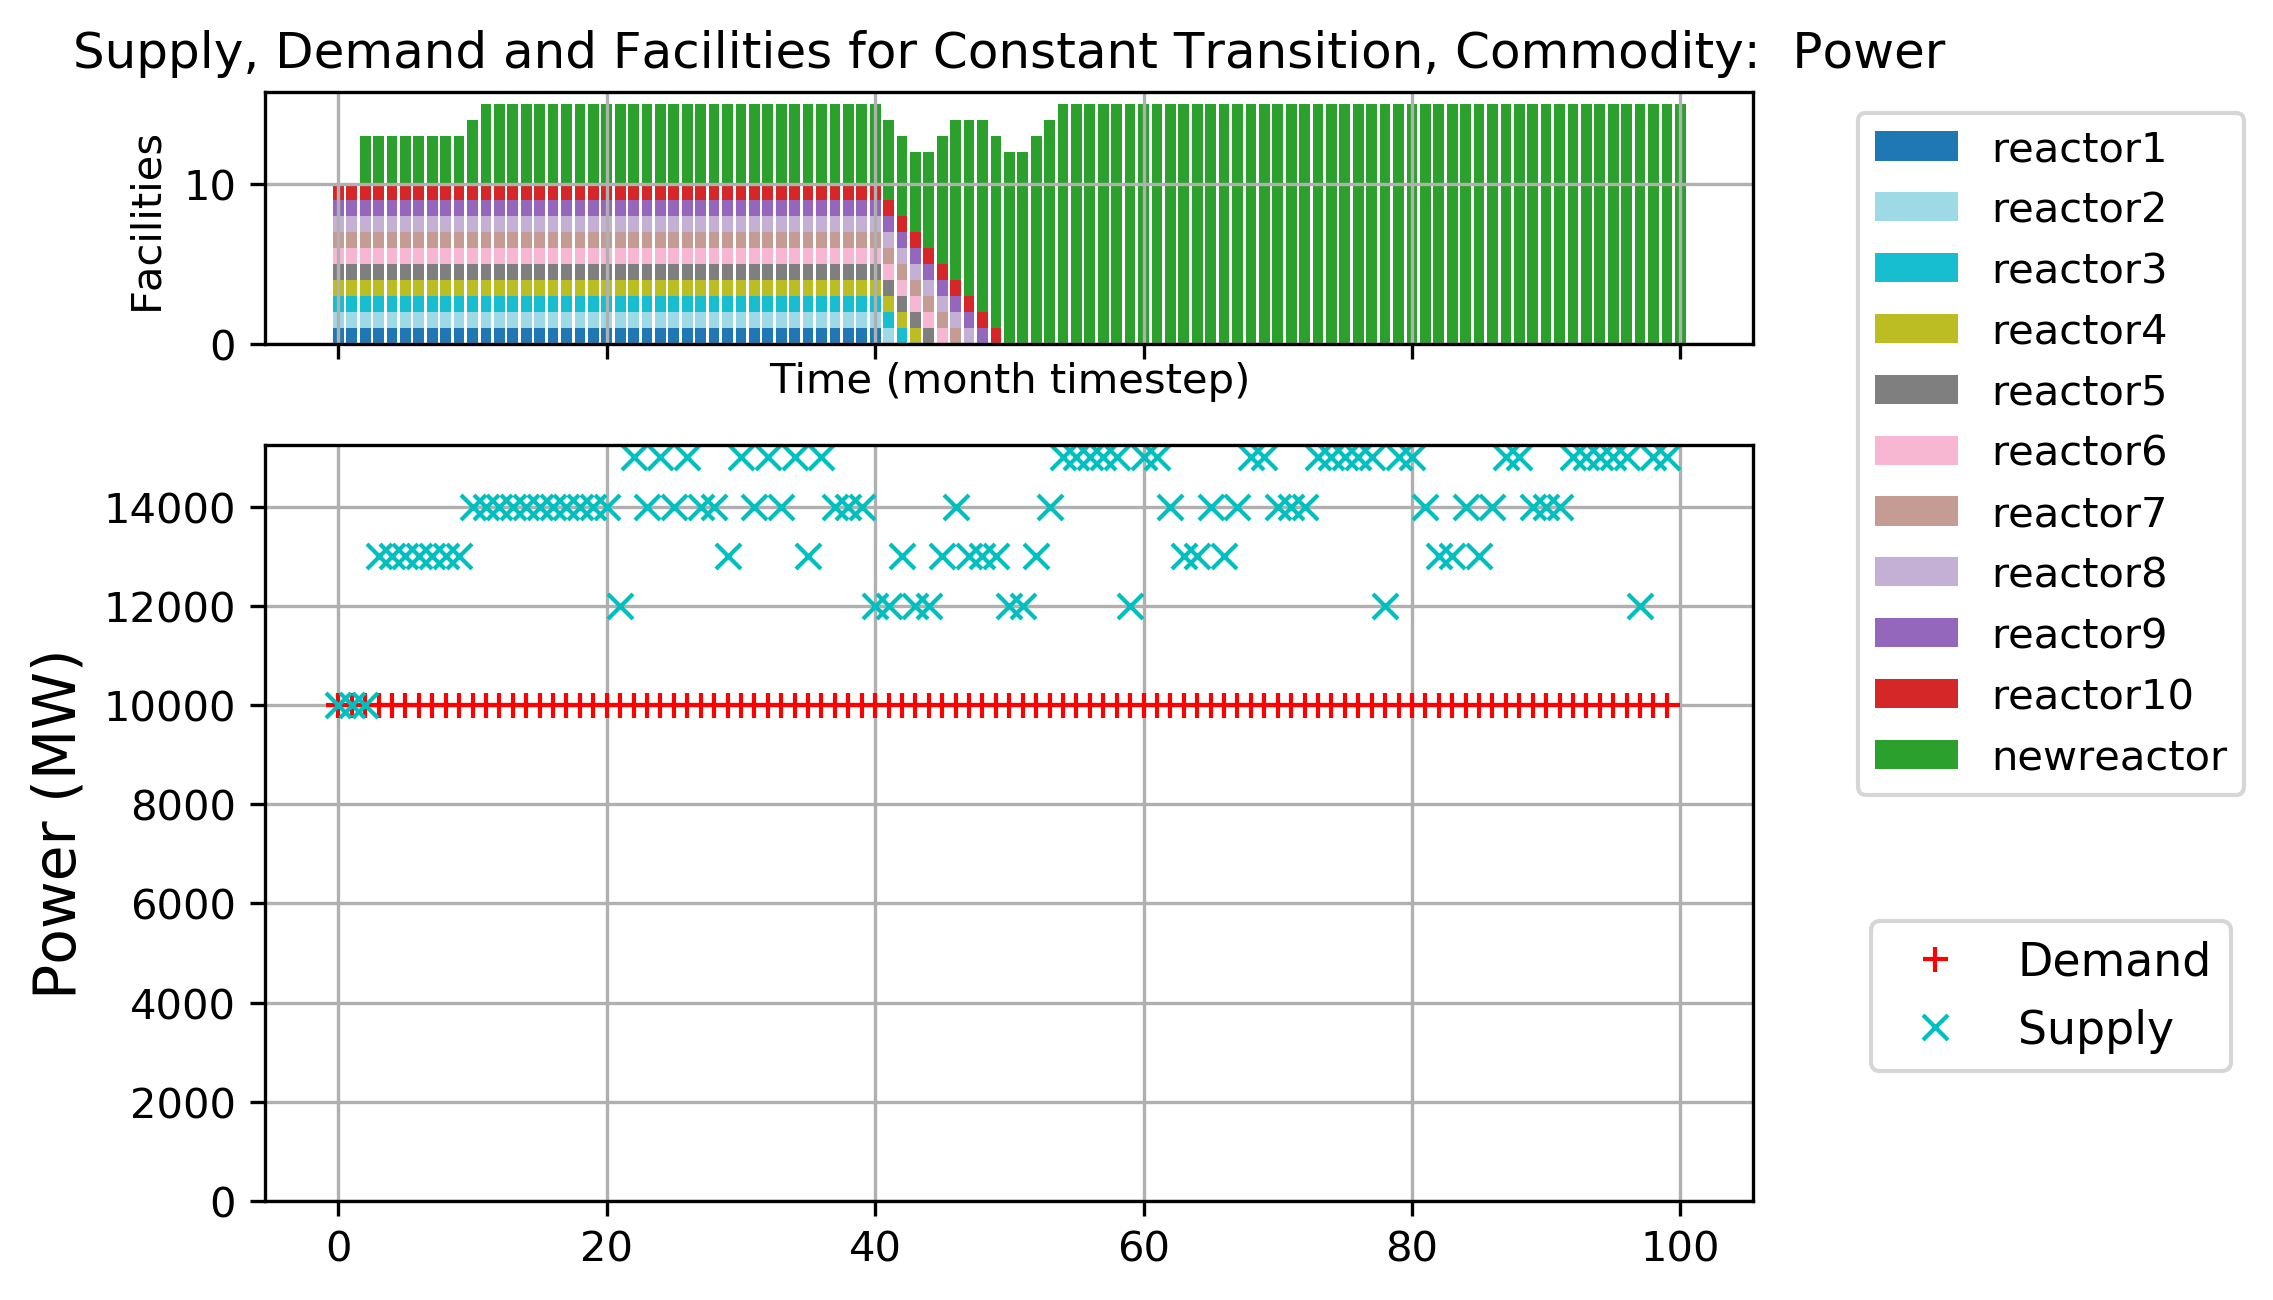
\includegraphics[width=0.9\linewidth]{figures/constanttransition-power.png} 
        \caption{Power demand and supply plot}
        \label{fig:constanttransition-power}
    \end{subfigure}
    \vspace{1cm}
    \begin{subfigure}[t]{0.45\textwidth}
        \centering
        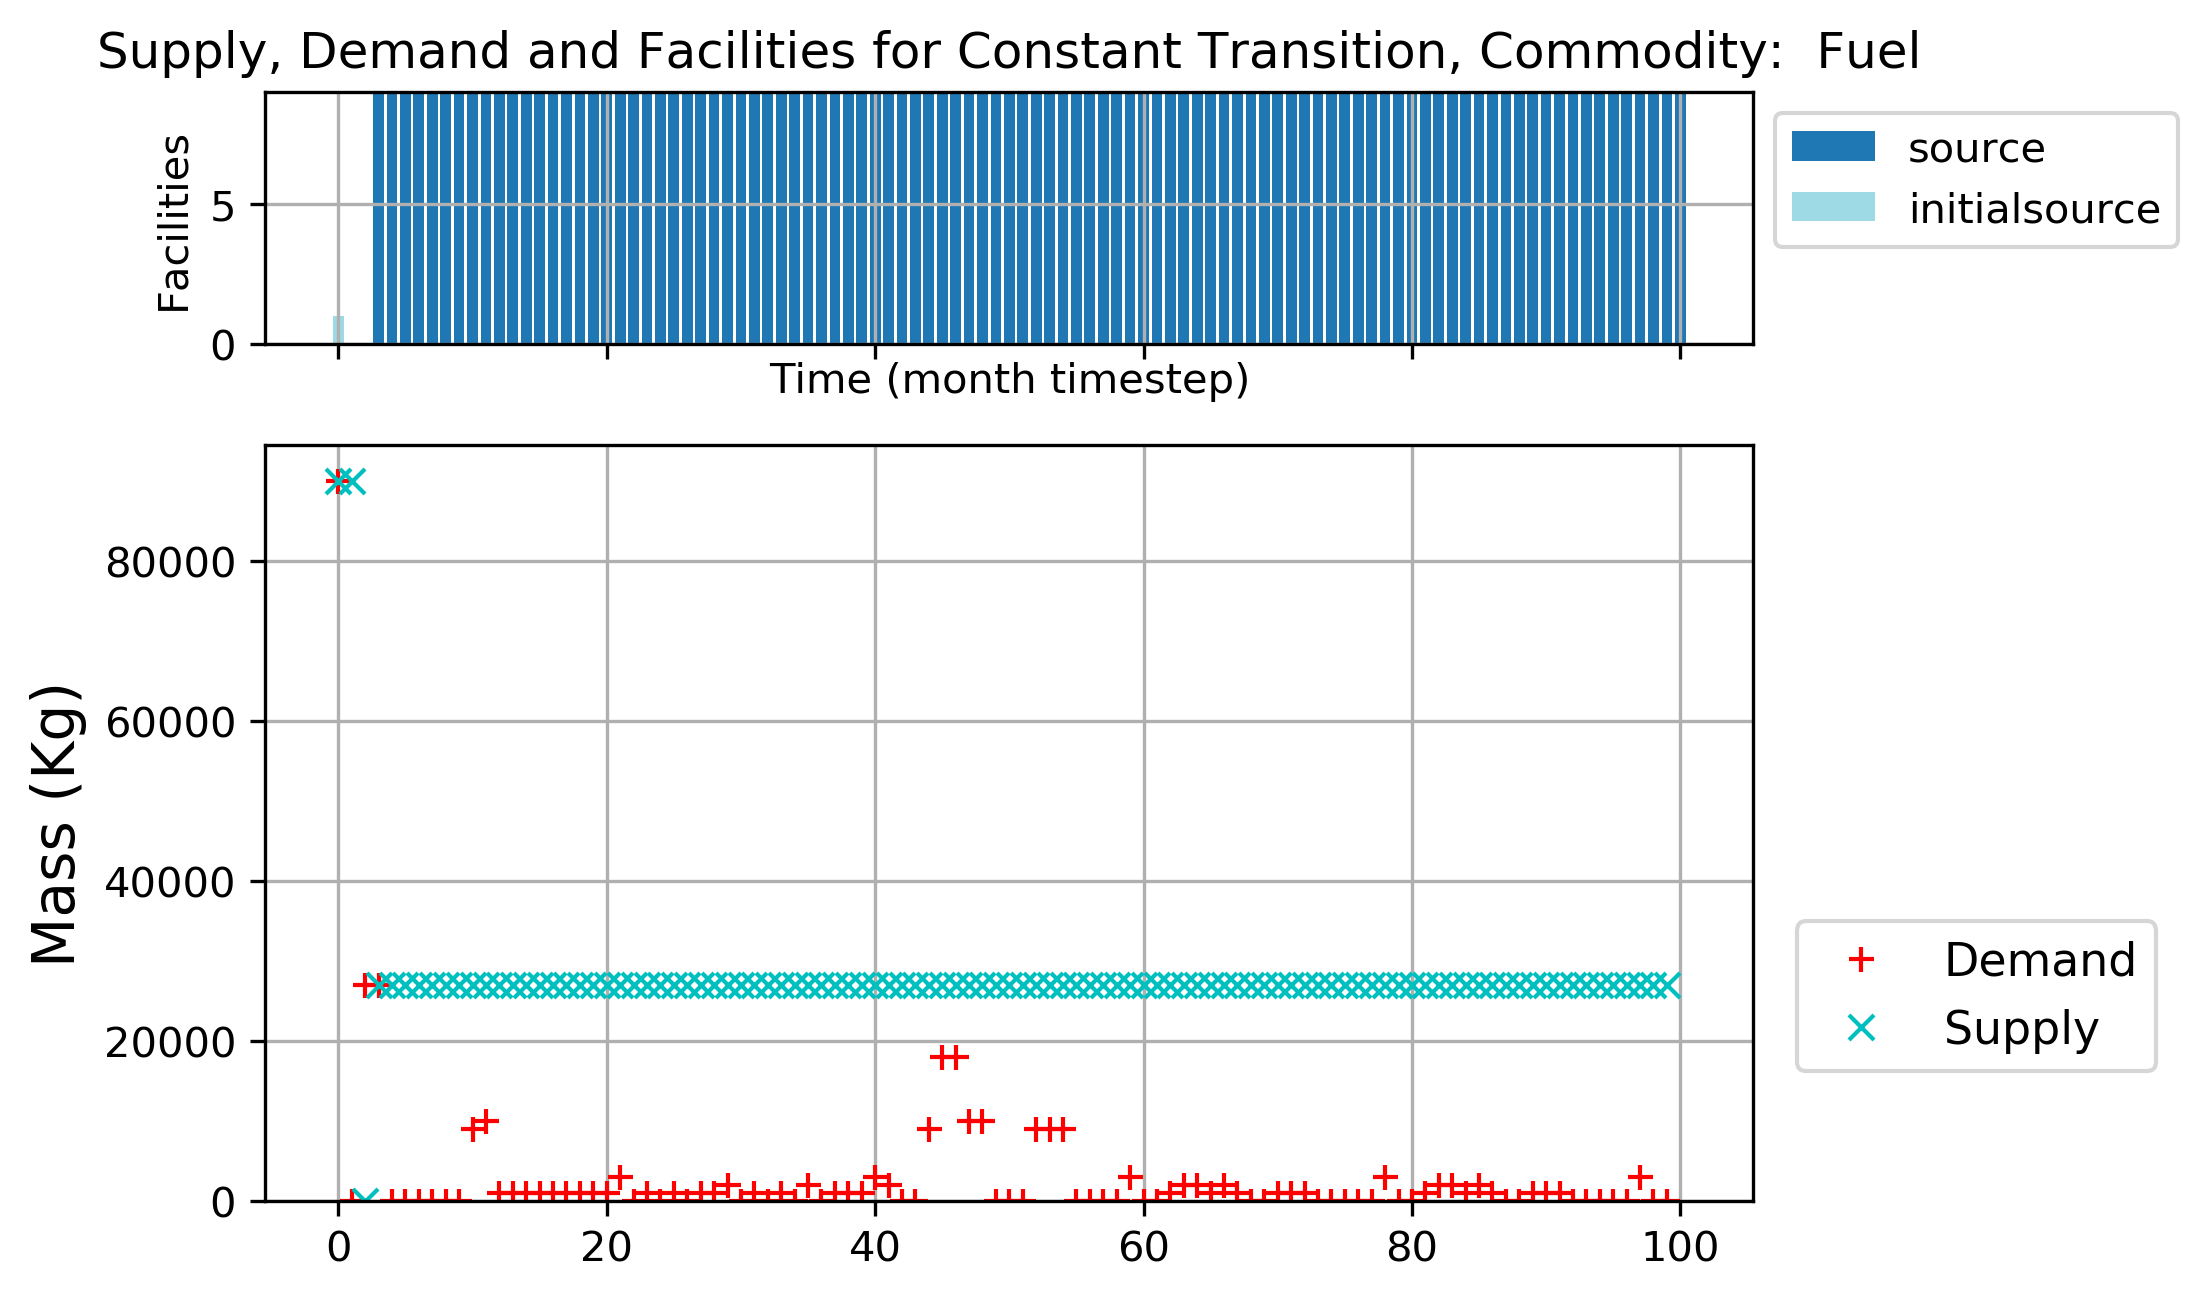
\includegraphics[width=\linewidth]{figures/constanttransition-fuel.png} 
        \caption{Fuel demand and supply plot}
	    \label{fig:constanttransition-fuel}
    \end{subfigure}
    \hfill
    \begin{subfigure}[t]{0.45\textwidth}
        \centering
        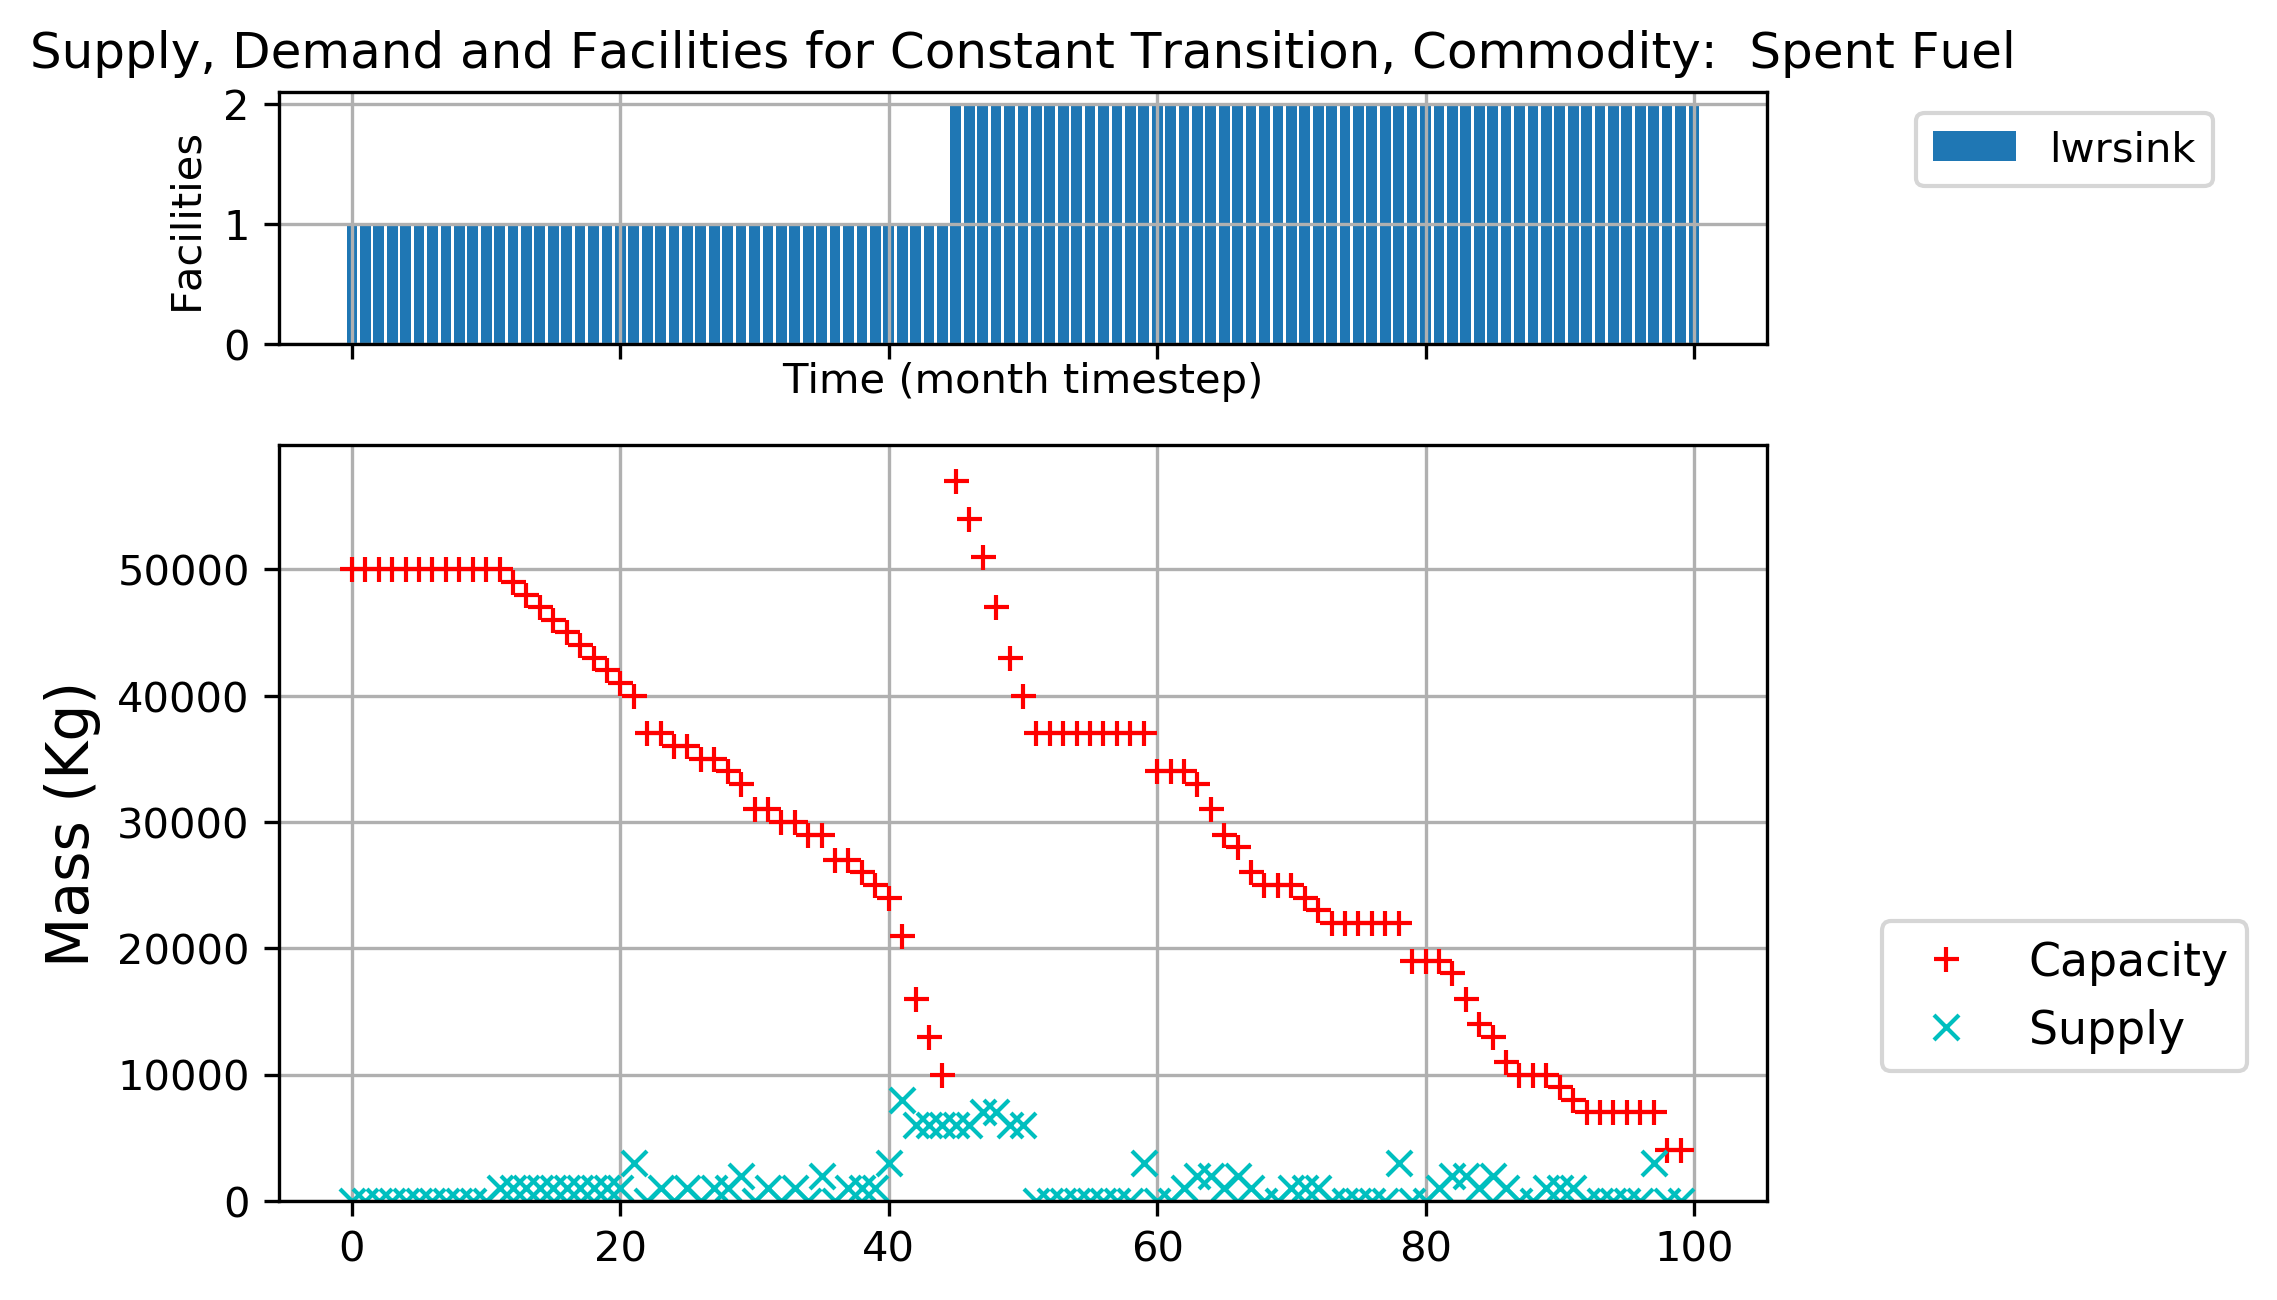
\includegraphics[width=\linewidth]{figures/constanttransition-spentfuel.png} 
        \caption{Spent Fuel demand and supply plot}
        \label{fig:constanttransition-spentfuel}
    \end{subfigure}
    \caption{Transition Scenario: Constant Power Demand of 10000MW}
\end{figure*}

\begin{table*}[htb]
    \centering
    \caption {Undersupply results for each commodity in each scenario}
	\label{tab:transition-scenario-results}
    \begin{tabular}{|l|l|p{4.5cm}|}
    \hline
    \textbf{Transition Scenario}    & \textbf{Commodity}    & \textbf{No. of time steps with undersupply} \\ \hline
    \multirow{2}{*}{\textbf{Constant Power}} & Fuel & 1 \\ \cline{2-3}
                                             & Power & 0 \\ \cline{2-3}
                                             & Spent Fuel & 0 \\ \hline
    \multirow{2}{*}{\textbf{Linearly Increasing Power}} & Fuel & 1 \\ \cline{2-3}
                                             & Power & 0 \\ \cline{2-3}
                                             & Spent Fuel & 0 \\ \hline
    \multirow{2}{*}{\textbf{Sinusoidal Power}} & Fuel & 1 \\ \cline{2-3}
                                             & Power & 1 \\ \cline{2-3}
                                             & Spent Fuel & 0 \\ \hline
    \end{tabular}
\end{table*}

In this section, a constant power transition scenario is shown. 
Recommendations and insights on specific parameters are 
discussed. 
Table \ref{tab:transition-scenario-constant-power} shows the 
simulation parameters used in this transition scenario. 

Figures \ref{fig:constanttransition-power}, \ref{fig:constanttransition-fuel}
and \ref{fig:constanttransition-spentfuel} demonstrate the capability 
of \deploy to deploy reactor and supporting facilities to meet the user 
determined power demand and subsequently demanded secondary commodities 
with minimal time steps where there is an undersupply. 
Table \ref{tab:transition-scenario-results} shows the number of time 
steps where there is undersupply for each commodity in this scenario. 
In figure \ref{fig:constanttransition-power}, there are no time steps
where the supply of power falls under demand.
A combination of using the fast fourier transform method for predicting 
demand and setting the supply buffer to 3000MW (the capacity of 3 reactors), 
the user is able to minimize the number of time steps where there 
is an undersupply of every commodity. 
It is important to perform a small sensitivity analysis of the size 
of buffer to use for each commodity to ensure that there is no 
undersupply based on the nuances of the facility type: 
refueling in a reactor etc. 

Figure \ref{fig:constanttransition-fuel} shows the demand and supply 
for fuel in the simulation. 
A facility with a large capacity of fuel is initially
deployed to meet the large initial fuel demand for the starting
up of ten reactors. 
By having an initial facility with a large throughput
to exist for the first few time steps in the simulation to meet 
the initial demand, 
\deploy is prevented from deploying a large amount of supporting
facilities that end up being redundant at the later parts of 
the simulation.   
This is a reflection of reality where reactor manufacturers will 
accumulate an appropriate amount of fuel inventory before starting 
up reactors. 
There is one time step where there is an undersupply after the 
decommissioning of the large initial facility.  
This is unavoidable the prediction methods in \deploy are unable 
to predict this sudden drop in demand. 


\subsection{\textbf{Transition Scenario: Linearly Increasing Demand}}

\begin{table*}[!htbp]
    \centering
    \caption {Linearly Increasing Power Demand Transition Scenario's Parameters}
	\label{tab:transition-scenario-growing-power}
    \begin{tabular}{|l|l|p{4.5cm}|}
    \hline
                                     & \textbf{Parameters}    & \textbf{Description} \\ \hline
    \textbf{Overall}& Demand Equation & Time<40: 10000 MW, Time>40: 250*t MW \\ \hline
    \multirow{2}{*}{\textbf{Power Commodity}} & Prediction Method      &  Fast Fourier Transform \\ \cline{2-3} 
                                     & Supply Buffer          &  2000 MW (2 reactor capacities)\\ \hline
    \multirow{2}{*}{\textbf{Fuel Commodity}}  & Prediction Method      &  Moving Average\\ \cline{2-3}
                                     & Supply Buffer & 1000 kg \\ \hline
    \multirow{2}{*}{\textbf{Spent Fuel Commodity}}  & Prediction Method      &  Fast Fourier Transform \\ \cline{2-3}
                                     & Capacity Buffer & 0 kg \\ \hline
    \end{tabular}
\end{table*}

\begin{figure*}[!htbp]
    \centering
    \begin{subfigure}[t]{\textwidth}
    \centering
        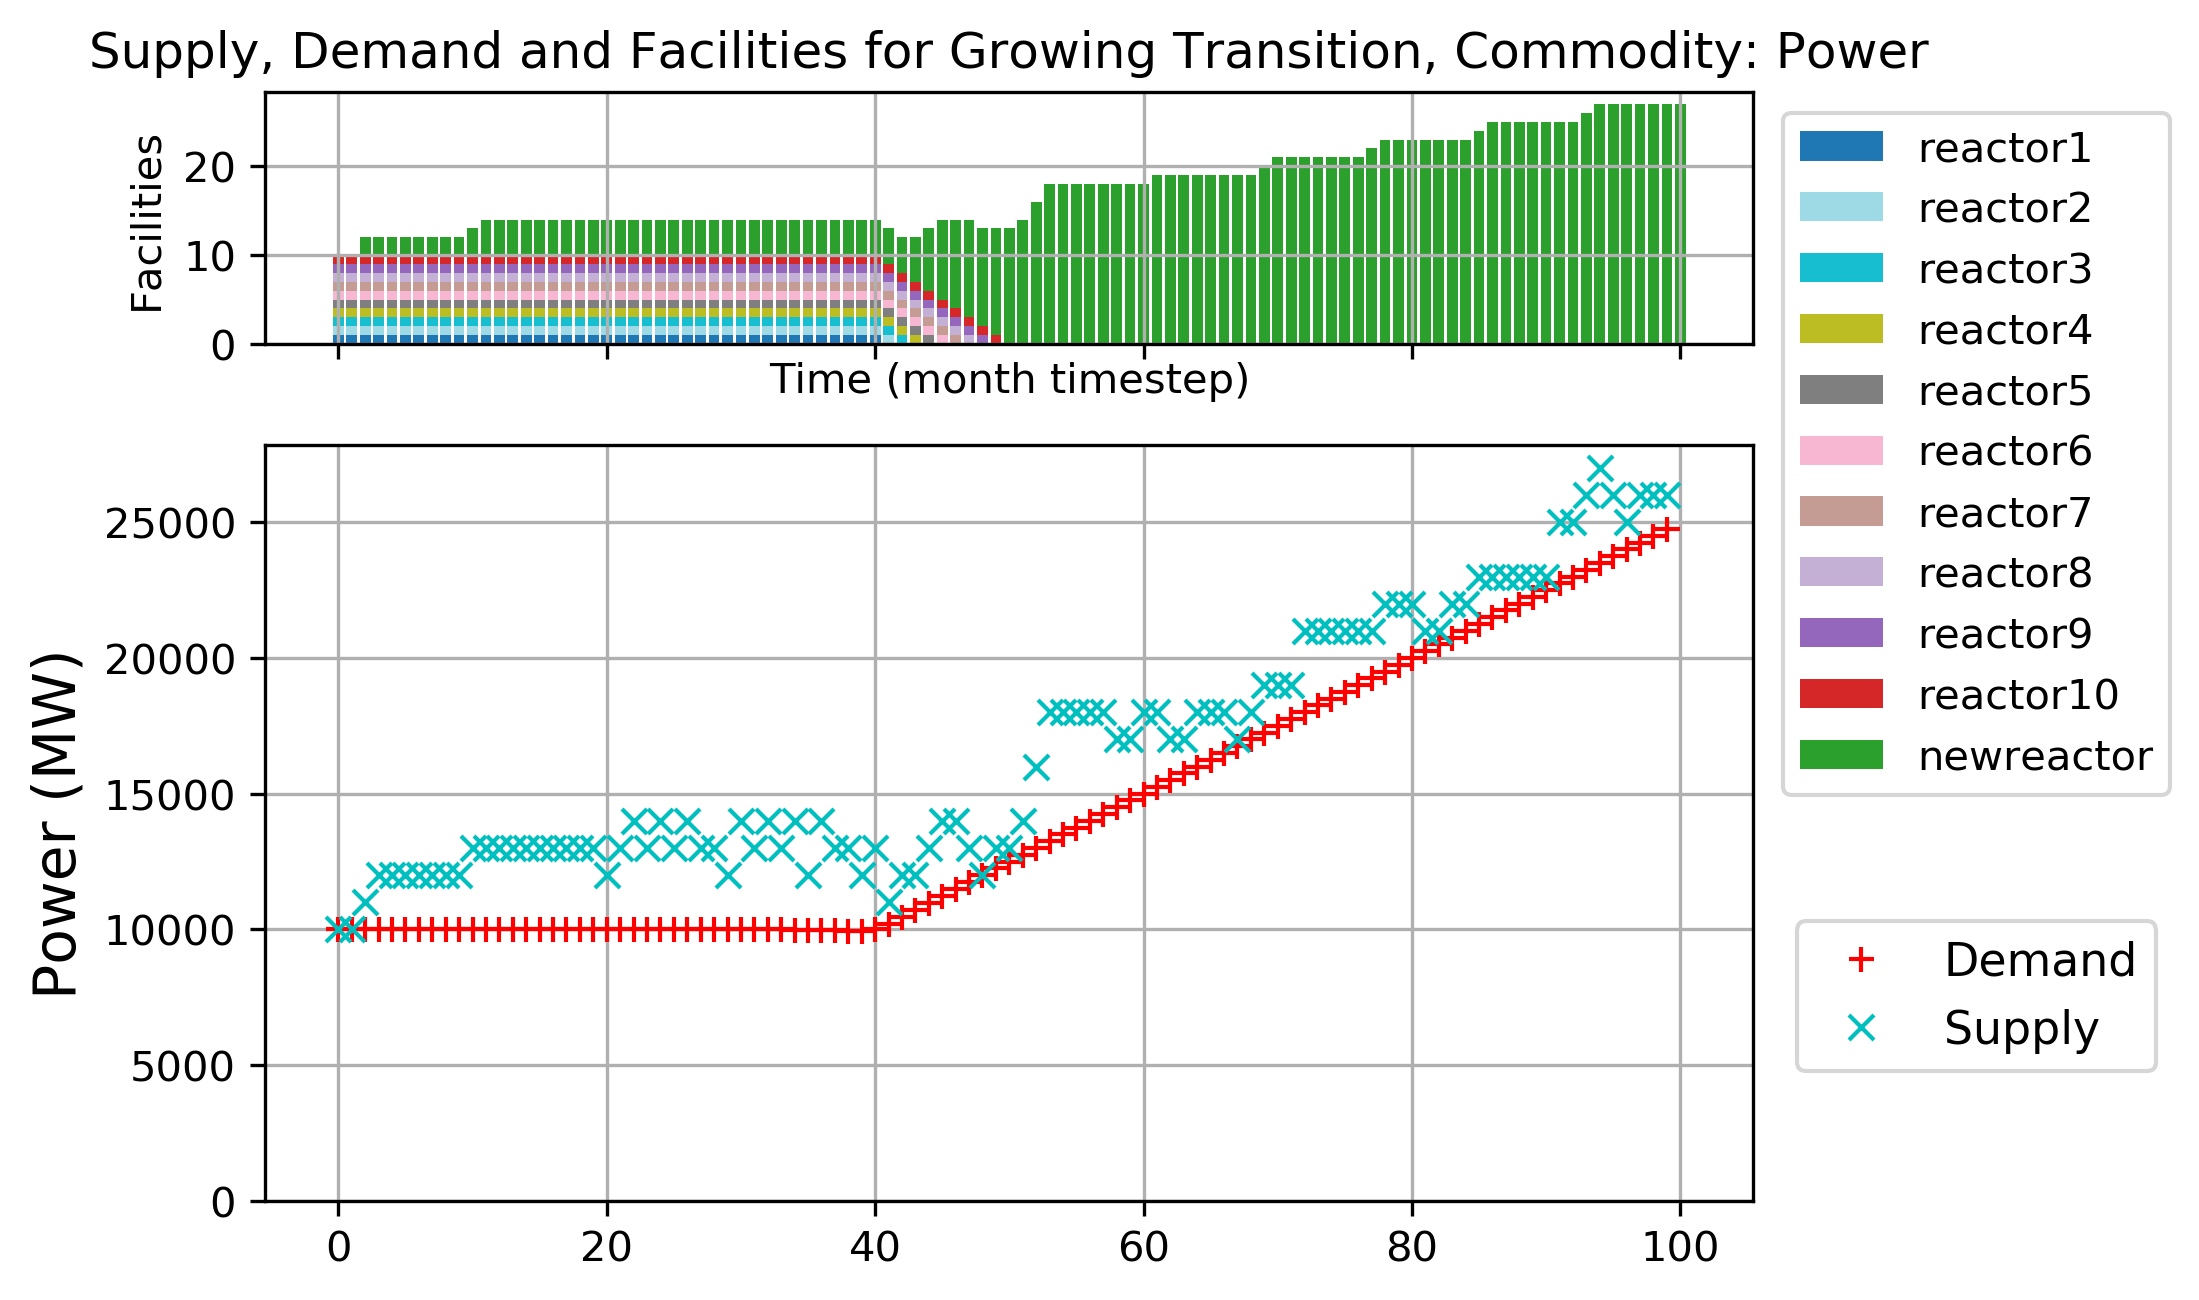
\includegraphics[width=0.9\linewidth]{figures/growingtransition-power.png} 
        \caption{Power demand and supply plot}
        \label{fig:growingtransition-power}
    \end{subfigure}
    \vspace{1cm}
    \begin{subfigure}[t]{0.45\textwidth}
        \centering
        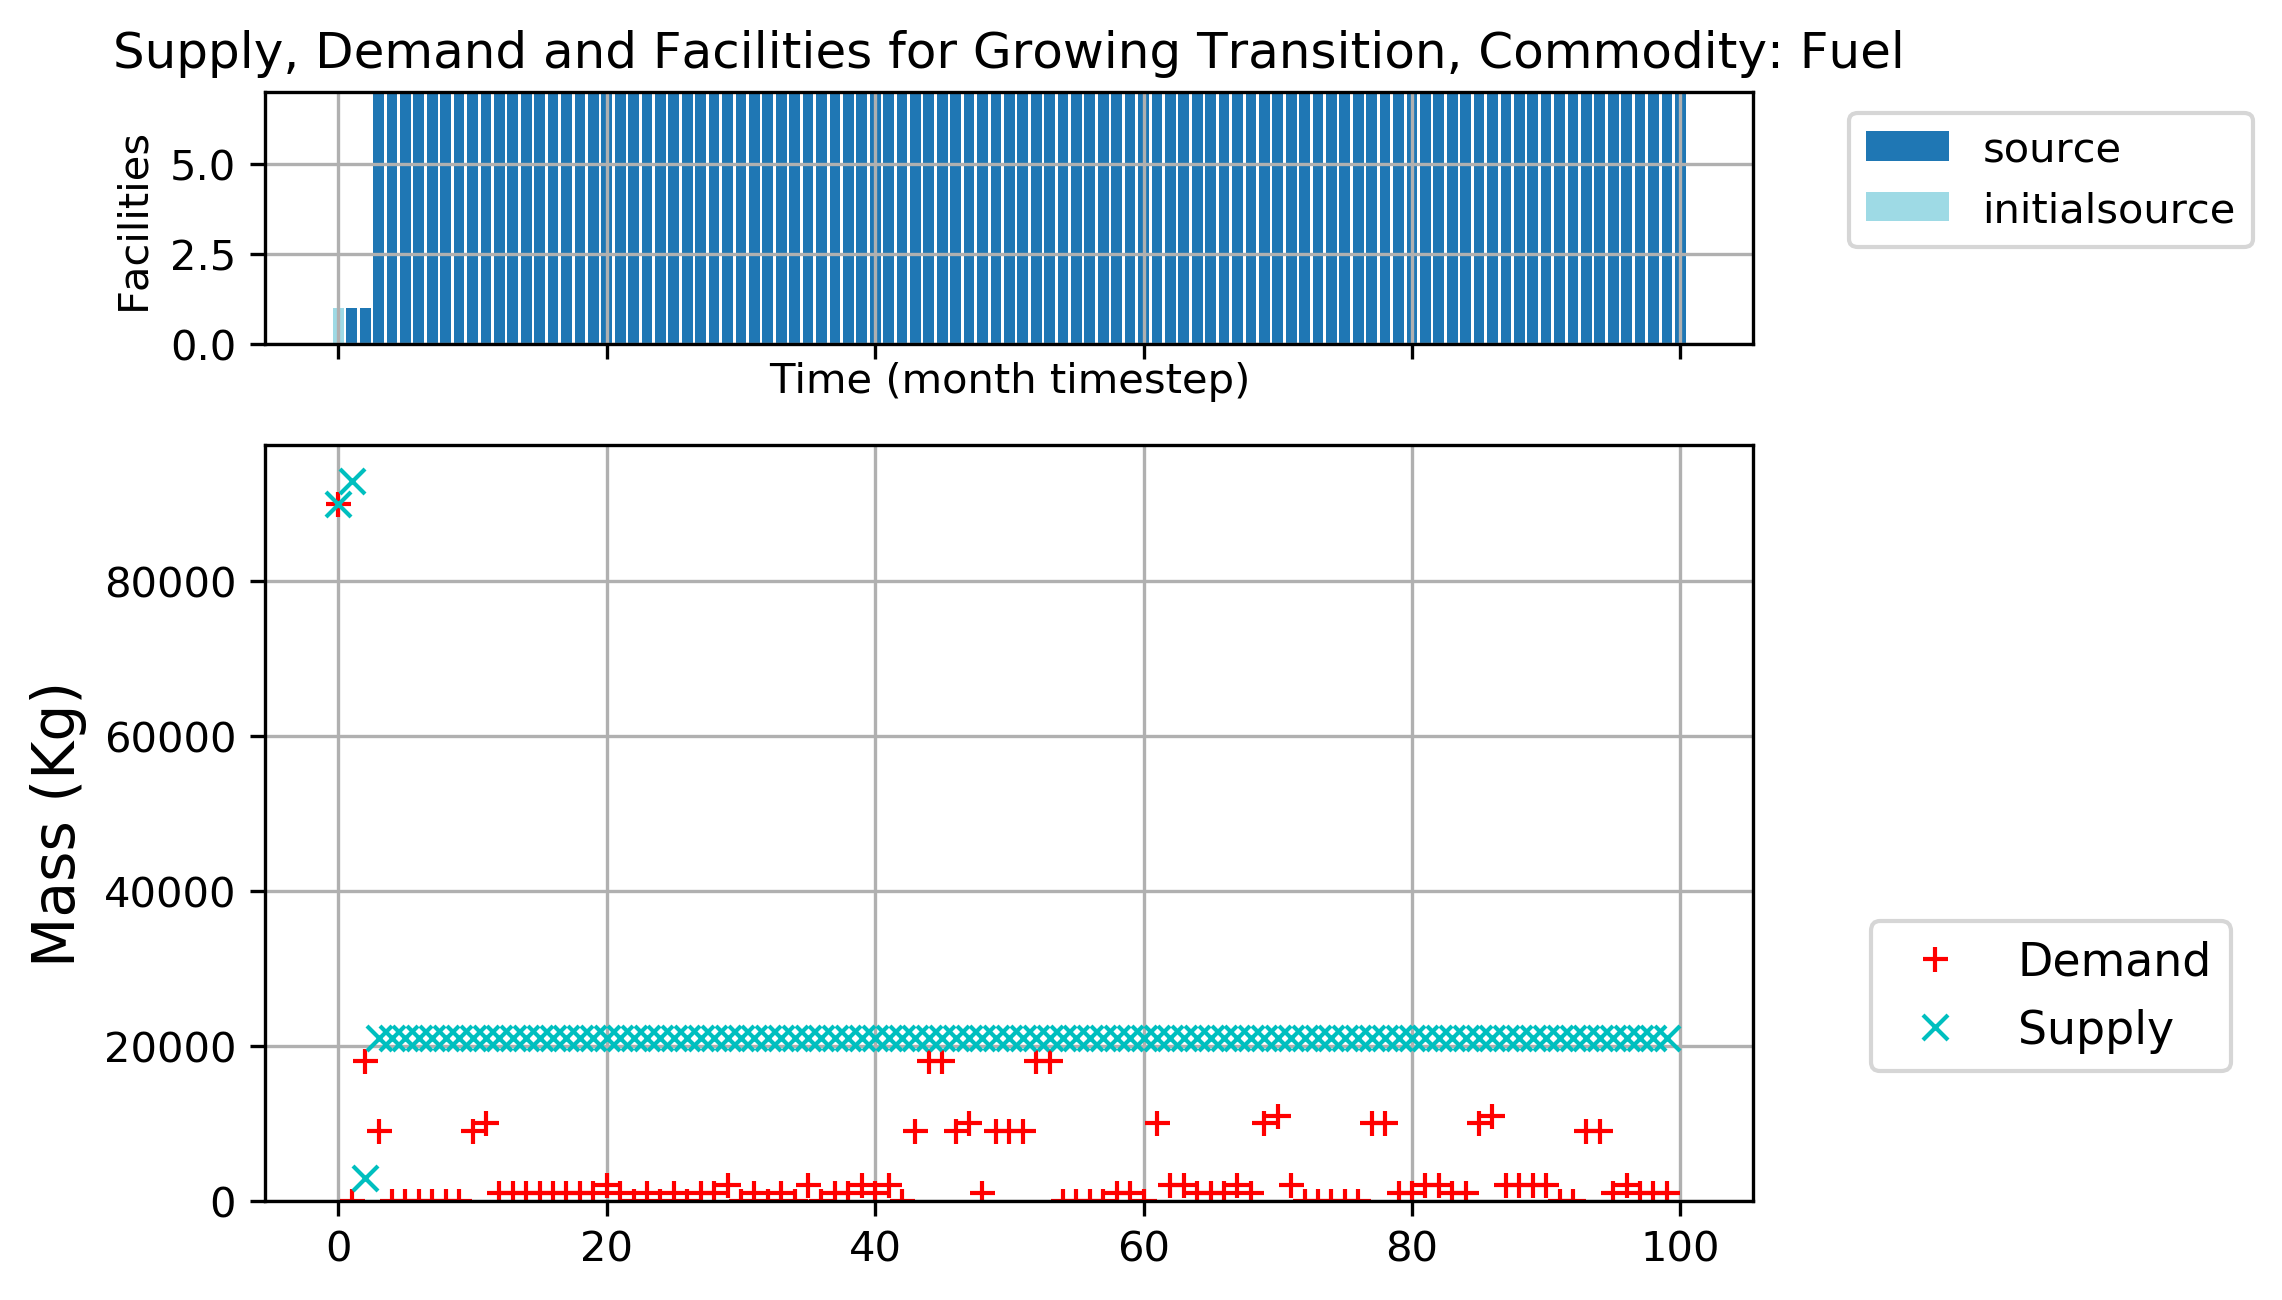
\includegraphics[width=\linewidth]{figures/growingtransition-fuel.png} 
        \caption{Fuel demand and supply plot}
	    \label{fig:growingtransition-fuel}
    \end{subfigure}
    \hfill
    \begin{subfigure}[t]{0.45\textwidth}
        \centering
        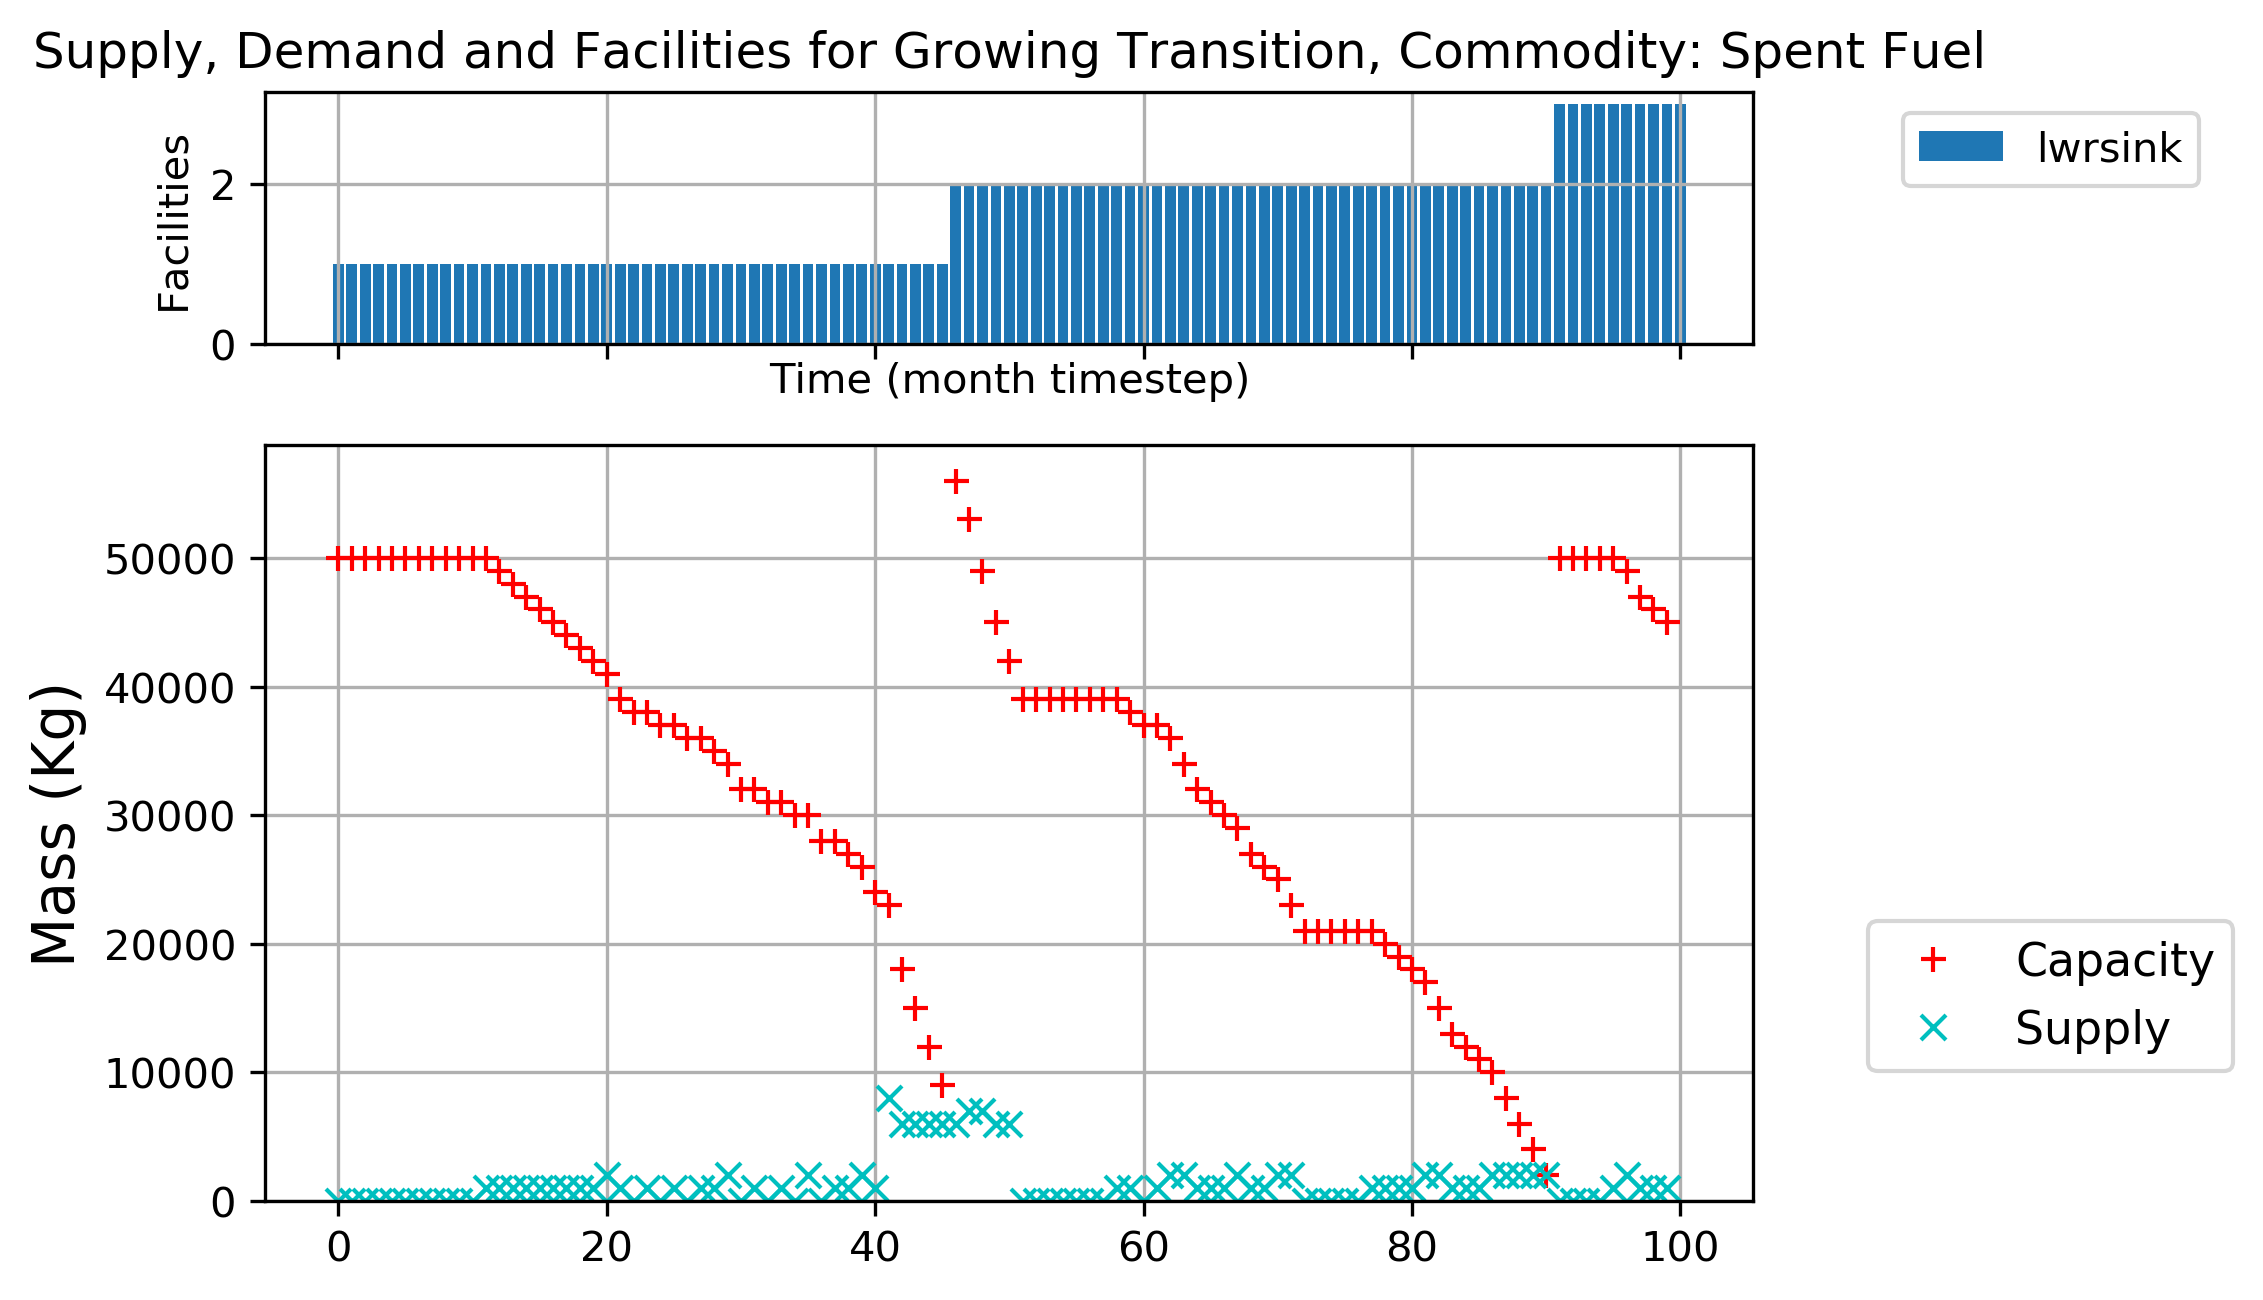
\includegraphics[width=\linewidth]{figures/growingtransition-spentfuel.png} 
        \caption{Spent Fuel demand and supply plot}
        \label{fig:growingtransition-spentfuel}
    \end{subfigure}
    \caption{Transition Scenario: Linearly Increasing Power Demand}
\end{figure*}

In this section, a transition scenario where there is a linearly 
increasing power demand is shown. 
Table \ref{tab:transition-scenario-growing-power} shows the 
simulation parameters used in this transition scenario. 

Figures \ref{fig:growingtransition-power}, \ref{fig:growingtransition-fuel}
and \ref{fig:growingtransition-spentfuel} demonstrate the capability 
of \deploy to deploy reactor and supporting facilities to meet the user 
determined power demand and subsequently demanded secondary commodities 
with minimal time steps where there is an undersupply for a linearly 
increasing power demand. 
For a linearly increasing power demand, the fast fourier 
transform method for predicting power demand is used 
which is similar to what was used for the constant power demand 
transition scenario. 
A smaller supply buffer for power was used. 

\subsection{\textbf{Transition Scenario: Sinusoidal Demand}}
In this section, a transition scenario where there is a sinusoidal
power demand is shown. 
A sinusoidal power demand is a reflection of the power demand in 
the real world where power usage is higher in the winter and summer
and is smaller in the spring and fall. 
Table \ref{tab:transition-scenario-sine-power} shows the 
simulation parameters used in this transition scenario. 

Figures \ref{fig:sinetransition-power}, \ref{fig:sinetransition-fuel}
and \ref{fig:sinetransition-spentfuel} demonstrate the capability 
of \deploy to deploy reactor and supporting facilities to meet the user 
determined power demand and subsequently demanded secondary commodities 
with minimal time steps where there is an undersupply for a sinusoidal 
power demand. 

For a sinusoidal power demand, the use of the triple exponential method
for predicting demand is more effective than the 
fast fourier transform method which was used for the constant 
and linearly increasing power demand transition scenarios. 
This is because the triple exponential smoothing method excels in
forecasting data points for repetitive seasonal series of data.  

\begin{table*}[!htbp]
    \centering
    \caption {Sinusoidal Power Demand Transition Scenario's Parameters}
	\label{tab:transition-scenario-sine-power}
    \begin{tabular}{|l|l|p{4.5cm}|}
    \hline
                                     & \textbf{Parameters}    & \textbf{Description} \\ \hline
    \textbf{Overall}& Demand Equation & time<40: 10000 MW, time>40: 250*t MW \\ \hline
    \multirow{2}{*}{\textbf{Power Commodity}} & Prediction Method      &  Triple Exponential Smoothing \\ \cline{2-3} 
                                     & Supply Buffer          &  2000 MW (2 reactor capacities)\\ \hline
    \multirow{2}{*}{\textbf{Fuel Commodity}}  & Prediction Method      &  Moving Average\\ \cline{2-3}
                                     & Supply Buffer & 0 kg \\ \hline
    \multirow{2}{*}{\textbf{Spent Fuel Commodity}}  & Prediction Method      & Fast Fourier Transform\\ \cline{2-3}
                                     & Capacity Buffer & 0 kg \\ \hline
    \end{tabular}
\end{table*}

\begin{figure*}[!htbp]
    \centering
    \begin{subfigure}[t]{\textwidth}
    \centering
        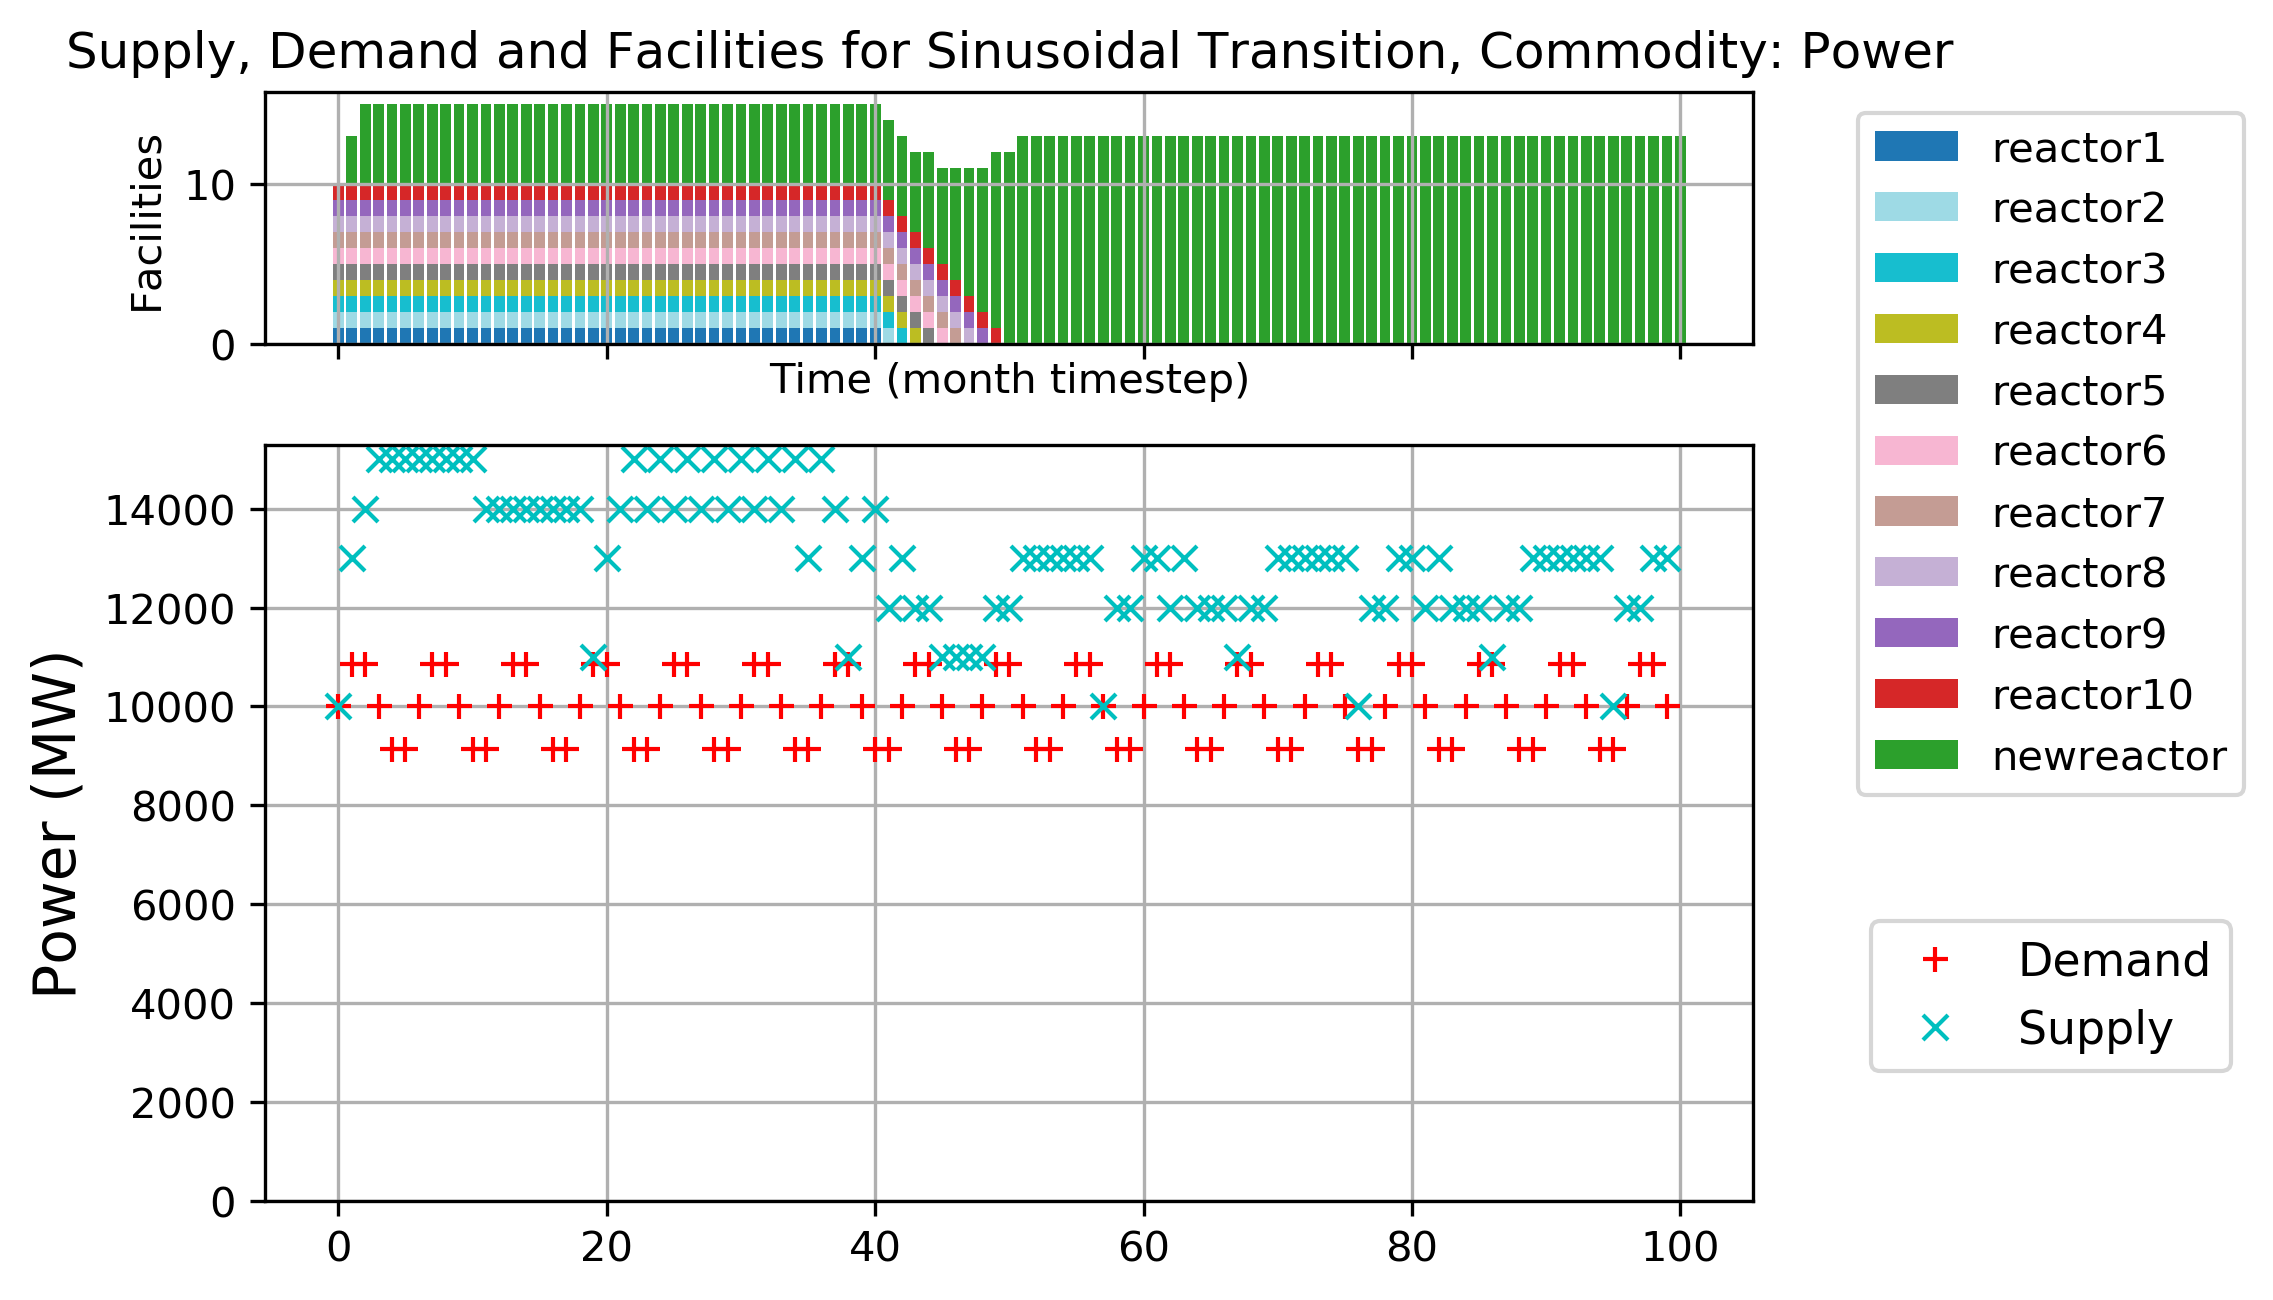
\includegraphics[width=0.9\linewidth]{figures/sinetransition-power.png} 
        \caption{Power demand and supply plot}
        \label{fig:sinetransition-power}
    \end{subfigure}
    \vspace{1cm}
    \begin{subfigure}[t]{0.45\textwidth}
        \centering
        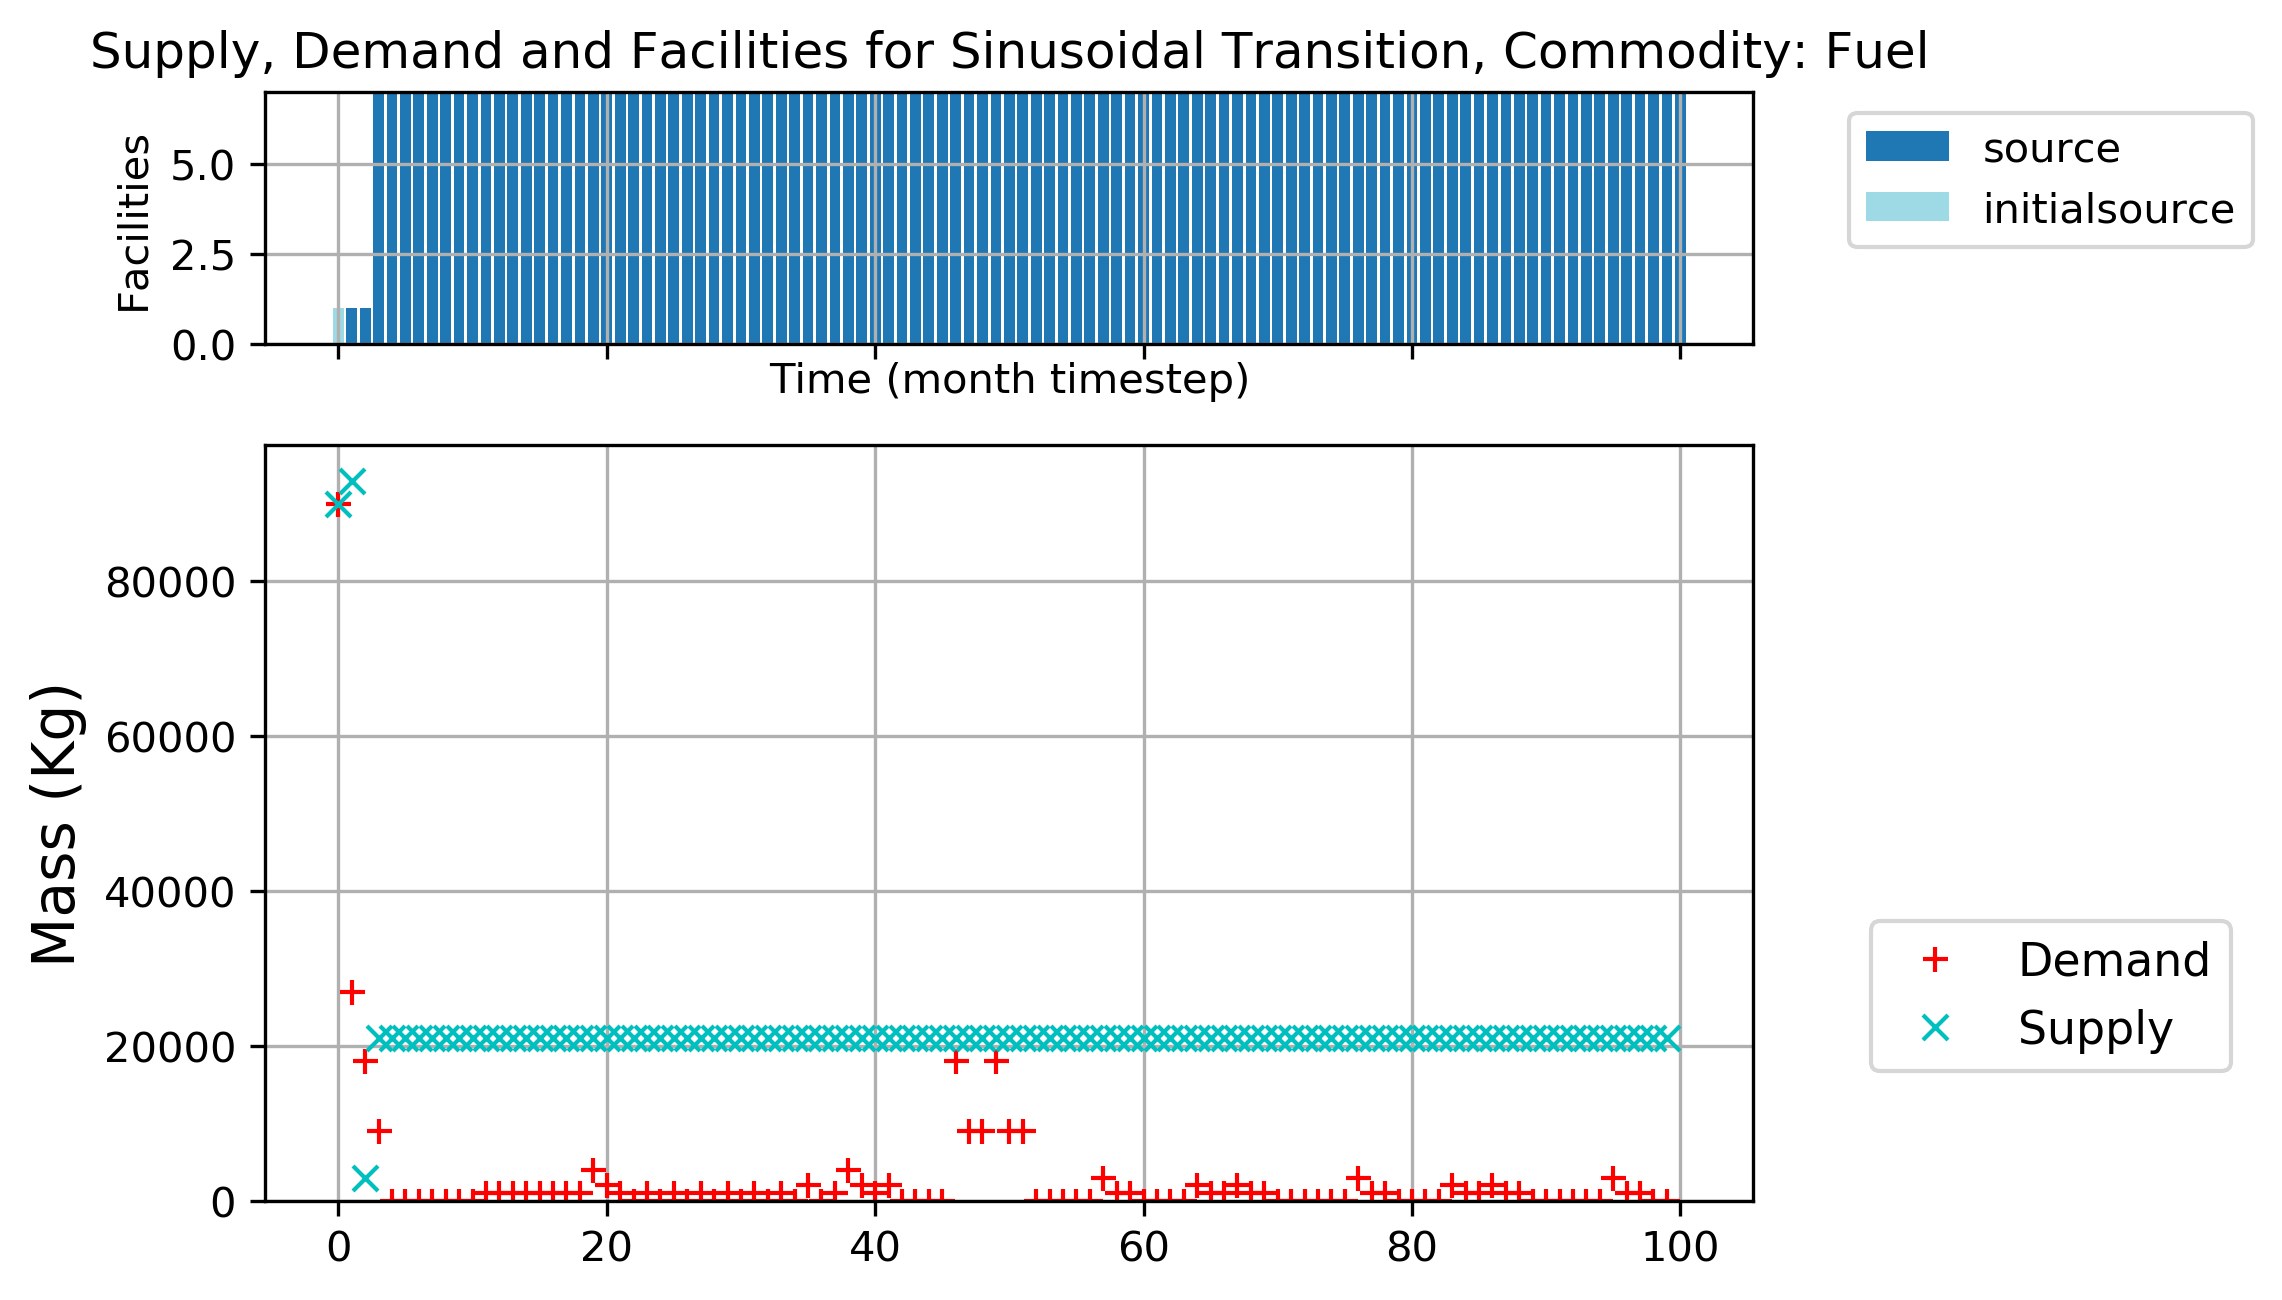
\includegraphics[width=\linewidth]{figures/sinetransition-fuel.png} 
        \caption{Fuel demand and supply plot}
	    \label{fig:sinetransition-fuel}
    \end{subfigure}
    \hfill
    \begin{subfigure}[t]{0.45\textwidth}
        \centering
        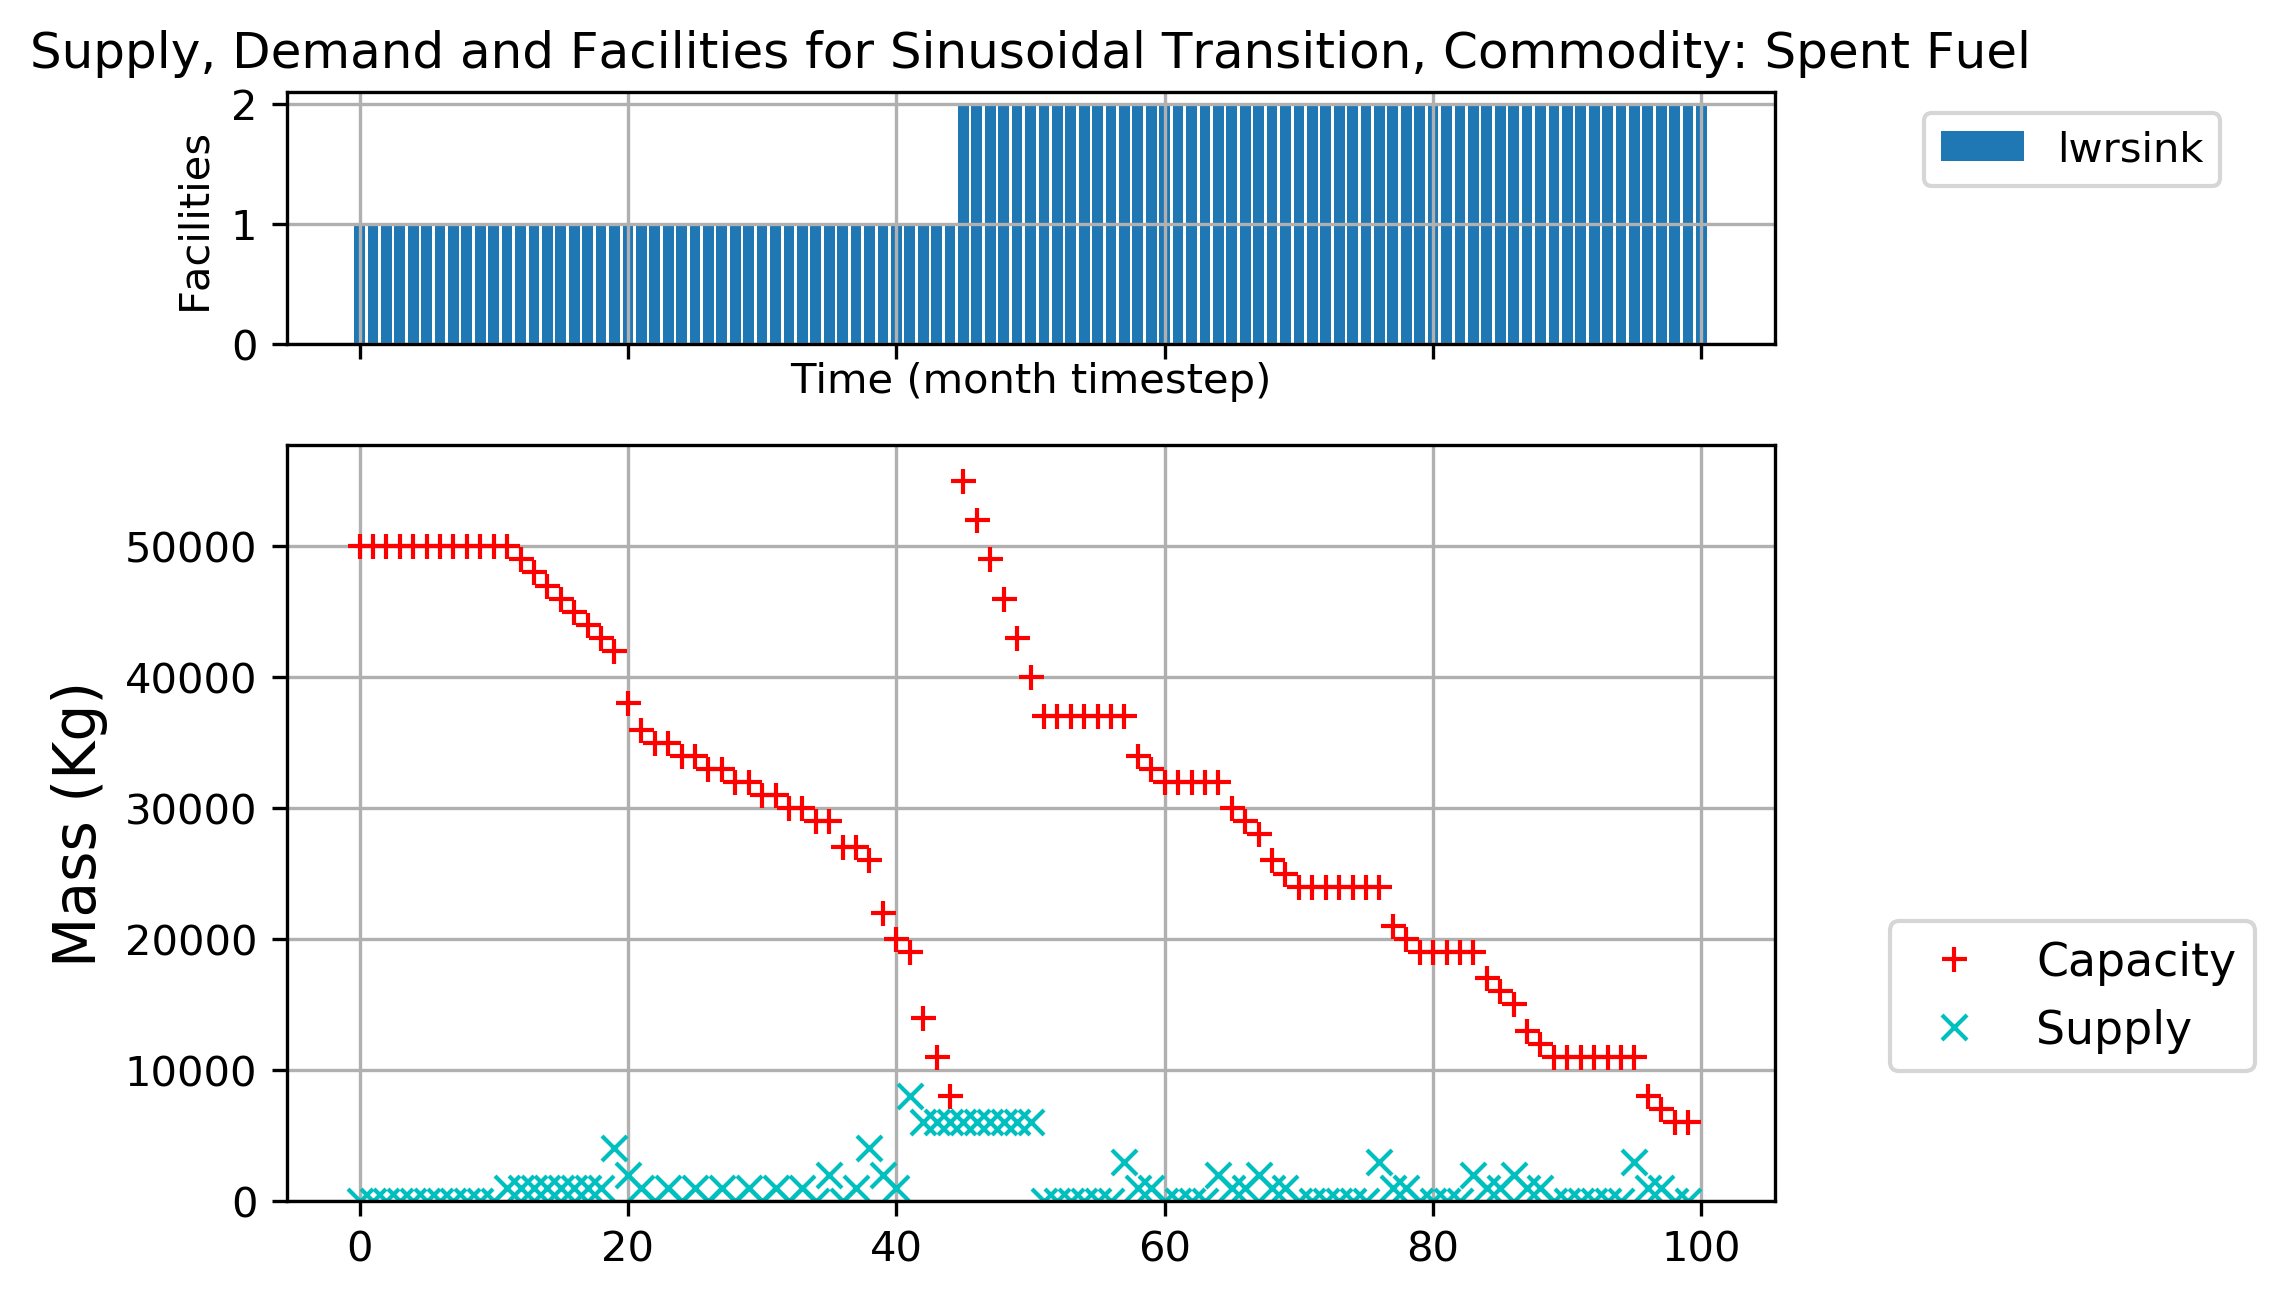
\includegraphics[width=\linewidth]{figures/sinetransition-spentfuel.png} 
        \caption{Spent Fuel demand and supply plot}
        \label{fig:sinetransition-spentfuel}
    \end{subfigure}
    \caption{Transition Scenario: Sinusoidal Power Demand}
\end{figure*}

%%%%%%%%%%%%%%%%%%%%%%%%%%%%%%%%%%%%%%%%%%%%%%%%%%%%%%%%%%%%%%%%%%%%
\section{Conclusion}
This paper describes the capabilities of \deploy, demonstrates 
the use of \deploy for an assortment of transition scenarios: 
constant power demand, linearly increasing power demand and
sinusoidal power demand.  
It also provides insights on parameter inputs when setting up larger
power demand transition scenarios that include many facilities. 
Future work includes setting up similar power demand transition 
scenarios for extended nuclear fuel cycles that incorporate reprocessing 
facilities etc. 
A more realistic transition scenario could be explored such as an 
increasing power demand that has a sinusoidal pattern to represent 
seasons in a year. 

\nopagebreak
%%%%%%%%%%%%%%%%%%%%%%%%%%%%%%%%%%%%%%%%%%%%%%%%%%%%%%%%%%%%%%%%%%%%
\section{Acknowledgements}
This research is funded by the \gls{DOE} Office of 
Nuclear Energy's Nuclear Energy University Program (Project 16-10512) 
"Demand-Driven Cycamore Archetypes". The authors want to thank 
members of the \gls{ARFC} group at the University of Illinois at 
Urbana-Champaign. 
We also thank our colleagues from the \Cyclus community, 
particularly those in the University of Wisconsin 
\gls{CNERG} and the University of South Carolina Energy Research 
Group (ERGS) for collaborative \Cyclus development.
%----------------------------------------------------------------%

%%%%%%%%%%%%%%%%%%%%%%%%%%%%%%%%%%%%%%%%%%%%%%%%%%%%%%%%%%%%%%%%%%%%
\bibliographystyle{ans}
\bibliography{bibliography}
\end{document}

